% -----------------------------------------------------------------
% Vorlage fuer Ausarbeitungen von
% Bachelor- und Masterarbeiten am ISS
% 
% Template for written reports or master theses at the ISS
% 
% For use with compilers pdflatex or latex->dvi2ps->ps2pdf.
%
% -----------------------------------------------------------------
% README, STUDENT USERS:
% We highly appreciate students using this template _AS IS_,period. 
% The document provides adjustable document preferences, 
% student information settings and typography definitions. Look for
% code delimited by *** ***
%
% The short explanation: it's the ISS common standard and 
% 	it's battle tested.
% The long explanation: 
%	We do not want you to go through the document and tweak the 
%	package options, layout parameters and line skips here and 
%	there and waste hours. We are providing this template such 
%	that you can fully concentrate on filling in the much more 
%	important _contents_ of your thesis.
%
% If you have serious needs on extra packages or design 
% modifications, talk to your supervisor _before_ modifying 
% the template.
% Similarly, we're happy if you give your supervisor a hint on any 
% errors in this template.
%
% -----------------------------------------------------------------
% History:
% Jan Scheuing,   04.03.2002
% Markus Buehren, 20.12.2004
% last changes:   10.01.2008 (removed unused packages), 
% 		07.08.2009 (added IEEEtran_LSS.bst file)
% 		02.05.2011 removed matriculation number from cover page
% Martin Kreissig, 25.01.2012: all eps/ps parts removed for 
% 				pdflatex to work properly
% Peter Hermannstaedter, 14.08.2012: fusion of versions for 
% 		latex/dvi/ps/pdf and pdflatex, additional comments,
% 		unification of document flags and student options
% Florian Liebgott, 12.03.2015: bug fixes, removal of obsolete options,
%		switch to UTF-8
% Florian Liebgott, 20.05.2015: fixed encoding problem on title page
% Florian Liebgott, 24.01.2017: changed deprecated font commands (like
%		\sl) to up-to-date commands to be compatible with
%		current TeX distributions.
% Felix Wiewel, 30.08.2021: Replace obsolete scrpage2 with scrlayer-scrpage
%
% -----------------------------------------------------------------
% If you experience any errors caused by this template, please
% contact Florian Liebgott (florian.liebgott@iss.uni-stuttgart.de)
% or your supervisor, so we can fix the errors.
% -----------------------------------------------------------------


\documentclass[12pt,DIV14,BCOR12mm,a4paper,footinclude=false,headinclude,parskip=half-,twoside,openright,cleardoublepage=empty,toc=index,bibliography=totoc,listof=totoc]{scrreprt}
% encoding needs to be defined here, otherwise umlauts on the titelpage won't work.
\newcommand{\fittable}[1]{%
  \begingroup
  \sbox0{\input{#1}}%
  \ifdim\wd0>\textwidth
    \resizebox{\textwidth}{!}{\usebox0}%
  \else
    \usebox0%
  \fi
  \endgroup
} 
\usepackage[utf8]{inputenc}
%
%
%
% *****************************************************************
% -------------------> document preferences here <-----------------
% *****************************************************************
% Uncomment the settings you like and comment the settings you don't
% like.

% Language: 
% affects generic titles, Figure term, titlepage and bibliography
% (Note:if you switch the language, compile tex and bib >2 times)
\def \doclang{english} 	% For theses/reports in English
%\def \doclang{german} 		% For theses/reports in German

% Hyperref links in the document:
\def \colortype{color} % links with colored text
%\def \colortype{bw} 	% plain links, standard text color (e.g. for print)
%\def \colortype{boxed} % links with colored boxes
% *****************************************************************
%
%
%
% *****************************************************************
% --------------> put student information here <------------------
% *****************************************************************
% Please fill in all items denoted by "to be defined (TBD)"
\def \deworktitle{Arbeitstitel, to be defined (TBD)}        % German title/translation
\def \enworktitle{Implementation of an Electromyography Processing Pipeline from Torch model to TinyML on resource-constrained microcontroller platforms}        % English title/translation
\def \tutor{Jonas Koellner, Prof. Dr Turker Ince}  % name of your supervisor
\def \student{Andrew Fady Fahmy}  % your name
\def \worksubject{Bachelorarbeit S1509}  % type and number (S/Dxxxx) of your thesis
\def \startdate{01/03/2026}
\def \submission{30/06/2026}
\def \signagedate{TBD Date of sign.}   % Date of signature of declaration on last page
\def \keywords{sEMG, TinyML, Digital Signal Processing, Deep Learning, regression,
 Limited-Resource Microcontroller Platforms} % keywords for your thesis
\def \abstract{Abstract TBD}

% *****************************************************************
%
\usepackage{tabularx}      % auto-width X column for the NN/SIMD text
\usepackage{makecell}      % \makecell and \shortstack for stacked cells
\usepackage{graphicx}      % \rotatebox for vertical headers
\usepackage{multirow}

\usepackage{amsmath}
\usepackage{amsfonts}
\usepackage{ifthen}

\usepackage{float}
\ifthenelse{\equal{\doclang}{german}}{
	\usepackage[ngerman]{babel} %german version
	\def \maintitle{\deworktitle}
	\def \translatedtitle{\enworktitle}
	% set , to decimal and . to thousands separator, if German language is used
	\DeclareMathSymbol{,}{\mathord}{letters}{"3B}
	\DeclareMathSymbol{.}{\mathpunct}{letters}{"3A}
	}{
	%english version
	\def \maintitle{\enworktitle}
	\def \translatedtitle{\deworktitle}
	}
\usepackage{txfonts} % Times-Fonts
\usepackage[T1]{fontenc}
\usepackage{color}
\usepackage[headsepline]{scrlayer-scrpage} % Headings

\usepackage{graphicx}
\usepackage[format=hang]{caption}       % for hanging captions
\usepackage{subfig}                     % for subfigures
\usepackage{wrapfig}                    % for figures floating in text, alternatively you can use >>floatflt<<
\usepackage{booktabs}                   % nice looking tables (for tables with ONLY horizontal lines)

%%%%% Tikz / PGF - drawing beautiful graphics and plots in Latex
% \usepackage{tikz}
% \usetikzlibrary{plotmarks}              % larger choice of plot marks
% \usetikzlibrary{arrows}                 % larger choice of arrow heads
% % ... insert other libraries you need
% \usepackage{pgfplots}
% % set , to decimal and . to thousands separator for plots, if German language is used
% \ifthenelse{\equal{\doclang}{german}}{
% \pgfkeys{/pgf/number format/set decimal separator={,}}
% \pgfkeys{/pgf/number format/set thousands separator={.}}
% }{}
%%%%%%

\ifthenelse{\equal{\colortype}{color}}{
	% colored text version:
	\usepackage[colorlinks,linkcolor=blue]{hyperref}
	\newcommand{\bugfix}{\color{white}{\texttt{\symbol{'004}}}} % Bug-Fix Umlaute in Verbatim
}{
	\ifthenelse{\equal{\colortype}{boxed}}{
		% colored box version:
		\usepackage{hyperref}
		\newcommand{\bugfix}{\color{white}{\texttt{\symbol{'004}}}} % Bug-Fix Umlaute in Verbatim
	}{
		% monochrome version:
		\usepackage[hidelinks]{hyperref}
		\newcommand{\bugfix}{\color{white}{\texttt{\symbol{'004}}}} % Bug-Fix Umlaute in Verbatim
	}
}

% Layout and Headings
\pagestyle{scrheadings}
\automark{chapter}
\clearscrheadfoot
\lehead[]{\pagemark~~\headmark}
\rohead[]{\headmark~~\pagemark}
\renewcommand{\chaptermark}[1]{\markboth {\normalfont\slshape \hspace{8mm}#1}{}}
\renewcommand{\sectionmark}[1]{\markright{\normalfont\slshape \thesection~#1\hspace{8mm}}}
\addtolength{\textheight}{15mm}
\parindent0ex
\setlength{\parskip}{5pt plus 2pt minus 1pt}
\renewcommand*{\pnumfont}{\normalfont\slshape} % Seitenzahl geneigt
\renewcommand*{\sectfont}{\bfseries} % Kapitelueberschrift nicht Helvetica

% Settings for PDF document
\pdfstringdef \studentPDF {\student} 
\pdfstringdef \worktitlePDF {\maintitle}
\pdfstringdef \worksubjectPDF {\worksubject}
\hypersetup{pdfauthor=\studentPDF, 
            pdftitle=\worktitlePDF,
            pdfsubject=\worksubjectPDF}

% Title page
\titlehead{
	
\includegraphics[width=20mm]{university-logo}
	\hspace{6mm}
	\ifthenelse{\equal{\doclang}{german}}{
		\begin{minipage}[b]{.6\textwidth}
		{\Large Universit\"at Stuttgart } \\
		Institut f\"ur Signalverarbeitung und Systemtheorie\\
		Professor Dr.-Ing. B. Yang \vspace{0pt}
		\end{minipage}
	}{
		\begin{minipage}[b]{.6\textwidth}
		{\Large University of Stuttgart } \\
		Institute for Signal Processing and System Theory\\
		Professor Dr.-Ing. B. Yang \vspace{0pt}
		\end{minipage}
	}
	\hspace{1mm}
	
\includegraphics[width=28mm]{isslogocolor}
}
\subject{\worksubject\vspace*{-5mm}} % Art und Nummer der Arbeit
\title{\maintitle}%\\ \Large{\subtitle}}
\subtitle{\translatedtitle}
\author{
\large
  \ifthenelse{\equal{\doclang}{german}}{
  \begin{tabular}{rp{7cm}}
    \Large 
    Autor:      & \Large \student \vspace*{2mm}\\
    Ausgabe:    & \startdate \\
    Abgabe:     & \submission \vspace*{3mm}\\
    Betreuer:   & \tutor \vspace*{2mm}\\
    Stichworte: & \keywords
  \end{tabular}
  }{
  \begin{tabular}{rp{7cm}}
    \Large 
    Author:             & \Large \student \vspace*{2mm}\\
    Date of work begin: & \startdate \\
    Date of submission: & \submission \vspace*{3mm}\\
    Supervisor:         & \tutor \vspace*{2mm}\\
    Keywords:           & \keywords
  \end{tabular}
  }
  \bugfix
}
\date{}
\publishers{\normalsize
  \begin{minipage}[t]{.9\textwidth}
    \abstract
  \end{minipage}
}

\numberwithin{equation}{chapter} 
\sloppy 

%
%
%
% *****************************************************************
% --------------> put typography definitions here <----------------
% *****************************************************************
% colors
\definecolor{darkblue}{rgb}{0,0,0.4}

% declarations
\newcommand{\matlab}{\textsc{Matlab}\raisebox{1ex}{\tiny{\textregistered}} }
% Integers, natural, real and complex numbers
\newcommand{\Z}{\mathbb{Z}}
\newcommand{\N}{\mathbb{N}}
\newcommand{\R}{\mathbb{R}}
\newcommand{\C}{\mathbb{C}}
% expectation operator
\newcommand{\E}{\operatorname{E}}
% imaginary unit
\newcommand{\im}{\operatorname{j}}
% Euler's number with exponent as parameter, e.g. \e{\im\omega}
\newcommand{\e}[1]{\operatorname{e}^{\,#1}}
% short command for \operatorname{}
\newcommand{\op}[1]{\operatorname{#1}}

% unknown hyphenation rules
\hyphenation{Im-puls-ant-wort Im-puls-ant-wort-ko-ef-fi-zien-ten
Pro-gramm-aus-schnitt Mi-kro-fon-sig-nal}
% *****************************************************************
%
\begin{document}

% title and table of contents
\pagenumbering{alph}
\maketitle
\cleardoublepage
\pagenumbering{roman} % roman numbering for table of contents
\tableofcontents
\cleardoublepage
\setcounter{page}{1}
\pagenumbering{arabic} % arabic numbering for rest of document

% *****************************************************************
% -------------------> start writing here <------------------------

\chapter{Basics and Foundations}
  \section{EMG and Deep Learning Pipelines for Bioelectric Signal Processing}
    \subsection{Bioelectric Signals and Human Machine Interaction (HMI)}

    Bioelectric signals are simply defined as a biological signal that originates
    from a human body, they are the sum of action potentials of cells at an anatomical site
    such as the heart, brain, or skeletal muscle  \cite{martinekAdvancedBioelectricalSignal2021}. These signals have been used extensively
    in Human Machine Interaction as they provide key insights about human's physiological activity as well as 
    presenting a more natural interaction medium between humans and computers. Although our primary focus in this
    work is about Electromyography (EMG) signals, we will frequently discuss other commonly researched bioelectric signals
    such as EEG (Electroencephalogram) and ECG (Electrocardiogram) signals given the abundance of useful Processing pipelines 
    and HMI research conducted using these 2 domains.

    \subsection{Electromyography (EMG) Basics}

    Electromyography is the recording of electrical activity in muscle. These electrical impulses originate
    from the spinal cord and propagate all the way to the peripheral nerves activating muscular contraction \cite{zhengSurfaceElectromyographyNatural2022}. 
    The motor neurons and the muscle fibers they innervate are defined as Motor Units which are recruited by these electrical impulses
    producing electrical signals. Professional electromyographers analyze characteristics features of these signals (i.e waveforms, firing rates, frequency of abrupt discharges, etc)
    deriving useful diagnostic information to identify abnormalities and different neural and muscle diseases

    The recording of EMG signals is mainly classified into two main categories. The first is intramuscular electromyography (iEMG) which is an invasive technique that
    includes inserting concentric needle electrodes inserted directly into muscle. The other is surface electromyography (sEMG) which is a non-invasive technique involving the placement of
    adhesive surface electrodes on skin surface. While iEMG has proven to be more effective in diagnosing medical conditions and abnormalities, sEMG dominate the HMI and gesture recognition
    sector due to its non-invasive nature, wider accessibility without the need of trained experts and user comfort \cite{valchevaSurfaceEMGDriven2026}. 

    In this study, we exclusively focus on sEMG data for the reasons mentioned above.

    \subsection{EMG Signal Preprocessing and Feature Extraction}
    Raw EMG signals suffer from a multitude of issues that obscure its insightful value.
    EMG signals are susceptible to various types of noise, which include electrical interference,
    physiological signals from adjacent muscles 
    that can contaminate the signal, the inherent instability of the signal,
    which arises because the firing rate of the motor units is itself
    quasi-random \cite{raezTechniquesEMGSignal2006} and obscure relevant information as well as
    movement artifacts and variations from one subject to another  
    \cite{valchevaSurfaceEMGDriven2026,coteallardDeepLearningElectromyographic2019}. 

    These problems clearly motivate extensive pre-processing steps to be taken in order to extract 
    as much insightful information as possible from EMG signals \cite{delucaFilteringSurfaceEMG2010}.Typically, sEMG signals recorded by commonly available sensors are in the range
    of $0$ to $400$ Hz. Band-pass butter worth filters of 4th order, with $20$--$450$~Hz range, 
    are used by most studies to retain viable information and discard the $5$-$20$~Hz corner frequencies\cite{delucaFilteringSurfaceEMG2010}.

    To filter out undesired high frequency noise. Many studies recommend the use of further smoothing algorithms
    like forward–backward filtering and the use of rectifiers to convert bipolar signal into positive-only
    mono-polar data. Normalization is also ubiquitous for digital signal processing and machine learning in order to 
    ensure steady and fast training times as well as reducing amplitude variability across subjects, sessions, and electrode placements 
    \cite{coteallardDeepLearningElectromyographic2019}.

    Windowing algorithms are widely adopted in EMG Preprocessing pipelines with varying parameter choices across the scientific literature.
    For real-time closed-loop control, input latency is critical: a maximum latency of $300$~ms was initially
    recommended \cite{hudginsNewStrategyMultifunction1993}, although more recent studies suggest that it should optimally be kept between $100$ and $250$~ms
    \cite{coteallardDeepLearningElectromyographic2019, smithDeterminingOptimalWindow2011}. While larger window sizes are preferred for higher quality
    models with better accuracy, smaller window sizes are the main choice for real-time systems and edge solutions that 
    prioritize faster performances and speed with limited resources.

    Feature extraction constitutes a further preprocessing stage emphasized
    across both research papers and textbooks. 
    Extracted features are categorized in DSP research into two main categories. Time Domain Features are features extracted from
    the filtered time-series data directly. Features like the mean absolute value (MAV), waveform length (WL),
    number of zero crossings (ZC), root mean square (RMS) are very widely adopted in research with varying successful 
    contributions from each. Frequency-domain features, by
    contrast, are derived from the Fourier transform of the time series and
    include measures such as the mean frequency (MNF) and peak frequency (PKF) \cite{phinyomarkFeatureReductionSelection2012}. 

    In this work, signal preprocessing is restricted to the time domain. The
    study adopts the increasingly prevalent paradigm that emphasizes feature
    learning through deep learning models rather than manual feature
    engineering, reflecting a broader shift in the field from feature
    engineering toward feature learning \cite{cote-allardInterpretingDeepLearning2020}.

    \subsection{Machine Learning and Deep Learning Approaches for sEMG-Based Classification and Regression}

    Approaches to sEMG decoding fall broadly into two paradigms: classical machine learning (ML) methods,
    which operate on hand-crafted features extracted from the signal, and deep learning (DL) methods, which
    learn task-relevant representations directly from the raw or minimally processed signal. This section
    surveys both, establishing the methodological context for the resource-constrained deployment that this
    thesis addresses.

    \subsubsection{Classical Machine Learning Approaches}

    Among classical ML classifiers, the Support Vector Machine (SVM) is one of the most widely adopted methods
    for sEMG-based gesture recognition \cite{niSurveyHandGesture2024}. An SVM constructs the decision boundary
    that maximises the margin separating the classes, where the margin is defined by the training examples
    lying closest to the boundary---the support vectors \cite{niSurveyHandGesture2024}. For data that are not
    linearly separable, which is typically the case for sEMG, the SVM employs the so-called kernel trick:
    rather than explicitly mapping the inputs into a higher-dimensional space in which a separating hyperplane
    exists, a kernel function (commonly the Radial Basis Function) computes the requisite inner products
    directly, thereby avoiding an explicit and costly nonlinear transformation \cite{niSurveyHandGesture2024}.

    SVMs have been applied extensively to sEMG classification, with feature-augmented variants reporting average
    accuracies as high as 99.98\% on constrained gesture sets \cite{t.HandGestureClassification2024}. The method
    is regarded as one of the more robust and accurate classical classifiers for sEMG
    \cite{mohapatraHandGestureClassification2024}, and is frequently employed as the reference baseline against
    which newly proposed sEMG decoders---including deep models intended for embedded
    deployment---are evaluated \cite{zanghieriRobustRealTimeEmbedded2020}. Other classical classifiers
    recurrently reported in the literature include Linear Discriminant Analysis (LDA), $k$-Nearest Neighbours
    (kNN), and Random Forests \cite{niSurveyHandGesture2024}, with comparative studies often finding LDA and SVM
    to yield broadly comparable accuracies on time-domain feature sets.

    The principal limitation shared by these classical methods is their dependence on a hand-crafted feature
    extraction and selection pipeline. Such pipelines require domain expertise to design, introduce subjectivity
    in the choice of features and parameters, and must frequently be re-tuned when signal characteristics change,
    which constrains their flexibility and generalisability \cite{niSurveyHandGesture2024}.

    \subsubsection{Deep Learning Approaches}

    Deep learning circumvents the manual feature-engineering bottleneck by learning hierarchical, task-relevant
    representations directly from the data, enabling end-to-end classification and regression
    \cite{zhongDeepFeatureLearning2026}. Owing to its successes across domains ranging from computer vision to
    digital signal processing, a broad repertoire of DL architectures has been adapted to sEMG decoding. Crucially,
    the choice of architecture is tightly coupled to the representation in which the sEMG signal is cast
    \cite{zhongDeepFeatureLearning2026}.

    When the multi-channel sEMG is arranged spatially---treating electrode channels as a spatial axis---it can be
    processed as an image, making Convolutional Neural Networks (CNNs) a natural and widely used choice, mirroring
    their dominance in image analysis \cite{zhongDeepFeatureLearning2026}. When instead the signal is treated as a
    set of temporal waveforms, sequence-modelling architectures become appropriate. Recurrent Neural Networks (RNNs)
    capture temporal dependencies by processing the sequence step by step, while their gated variants---the Long
    Short-Term Memory (LSTM) and the Gated Recurrent Unit (GRU)---introduce memory cells and gating mechanisms that
    mitigate the vanishing and exploding gradient problems, thereby improving the modelling of long-range temporal
    dependencies \cite{zhongDeepFeatureLearning2026}.

    Temporal Convolutional Networks (TCNs) have more recently emerged as a compelling alternative to recurrent
    models for sEMG sequence modelling. Because they apply convolutions along the time axis, TCNs process entire
    segments in parallel rather than sequentially, affording greater training efficiency and scalability than RNNs
    \cite{zhongDeepFeatureLearning2026}. Through dilated causal convolutions, a TCN can expand its receptive
    field---and thus the temporal context it captures---exponentially with depth, without a commensurate increase
    in parameter count \cite{zanghieriRobustRealTimeEmbedded2020, zhongDeepFeatureLearning2026}. These properties
    have made TCNs particularly attractive for real-time, resource-constrained sEMG decoding, a point developed
    further in the subsequent discussion of embedded and TinyML solutions.

  \section{TinyML and Resource-Constrained Microcontroller Platforms} 
    \subsection{Microcontrollers}
    A microcontroller unit (MCU) is a self-contained computing system integrated onto a single chip. 
    It comprises the core components required for general-purpose computation, including a central processing unit (CPU), volatile memory (RAM),
    non-volatile FLASH storage, and input/output (I/O)
    peripherals. The adoption of MCUs has accelerated markedly in recent years, driven largely by the proliferation of IoT systems (Internet of Things),
    which deploy numerous interconnected devices to acquire, process, and extract actionable insights from on-ground sensor data, transmitting this
    information across dedicated channels and networks for subsequent processing and decision-making.

    The contemporary MCU market is served by several prominent vendors, including Arduino (notably the UNO and Nano modules), Espressif Systems (the ESP32
    family), and STMicroelectronics (the STM32 series), among others. This landscape continues to evolve rapidly as new architectures and capabilities emerge.

    \subsection{Limitations and Constraints of Microcontroller Platforms}
    The low cost, compact form factor, and minimal power consumption that characterise MCUs are achieved through significant trade-offs relative to
    general-purpose and high-performance computing platforms.

    Foremost among these is severely constrained memory \cite{yelchuriReviewTinyML2022}.
    On-chip memory is approximately three orders of magnitude smaller than that of mobile devices, and five to six orders of magnitude smaller than that of
    cloud-based GPUs \cite{linMCUNetTinyDeep2020}.
    Clock frequencies are similarly limited, typically operating in the megahertz (MHz) range, in contrast to the gigahertz (GHz) range of modern
    general-purpose processors. A further constraint is the absence of GPUs or dedicated parallel processing units, which restricts the efficient execution
    of single-instruction-multiple-data (SIMD) operations and vectorised computation; this limitation has historically impeded the adoption of MCUs in the
    graphics and machine learning domains. Moreover, software development for MCUs remains notoriously cumbersome, owing to fragmented vendor-specific SDKs
    and frameworks, the prevalent reliance on deprecated software to accommodate hardware constraints, and the limited continuity of support and maintenance
    for development toolchains.

    
    % =====================================================================
%  MCU comparison table  --  requires in preamble:
%      \usepackage{booktabs}
%      \usepackage{tabularx}
%  Include in the main document with:   \input{mcu_comparison_table}
% =====================================================================
\begin{table}[htbp]
    \centering
    \caption{Comparison of commercially available MCUs for edge ML applications.}
    \label{tab:mcu_comparison}
    \renewcommand{\arraystretch}{1.25}
    \footnotesize
    \setlength{\tabcolsep}{4pt}
    % Three flexible (X) columns share the leftover width equally.
    \begin{tabularx}{\textwidth}{@{}l >{\raggedright\arraybackslash}X c >{\raggedright\arraybackslash}X >{\raggedright\arraybackslash}X c@{}}
        \toprule
        \textbf{MCU} & \textbf{Processor} & \textbf{WiFi/BT}
            & \textbf{Memory \& FPU} & \textbf{NN / SIMD} & \textbf{Cost} \\
        \midrule
        ESP32
            & Xtensa LX6, 2$\times$ @\,240\,MHz
            & Yes
            & 520\,KB SRAM; 8\,MB PSRAM + 16\,MB Flash (ext.); SP~FPU
            & ESP-DL / ESP-NN
            & \$3--8 \\
        \addlinespace[3pt]
        ESP32-S3
            & Xtensa LX7, 2$\times$ @\,240\,MHz
            & Yes
            & 512\,KB SRAM; 8\,MB PSRAM + 16\,MB Flash (ext.); SP~FPU
            & ESP-DL / ESP-NN (vector ext.)
            & \$4--10 \\
        \addlinespace[3pt]
        Pi Pico (RP2040)
            & Cortex-M0+, 2$\times$ @\,133\,MHz
            & Wi-Fi\textsuperscript{a}
            & 264\,KB SRAM; ext. PSRAM; 2\,MB Flash; no FPU
            & CMSIS-NN (no SIMD)
            & \$4--6 \\
        \addlinespace[3pt]
        Arduino Nano
            & ATmega328P (8-bit), 1$\times$ @\,16\,MHz
            & No
            & 2\,KB SRAM; no PSRAM; 32\,KB Flash; no FPU
            & None
            & \$10--25 \\
        \addlinespace[3pt]
        STM32H7
            & Cortex-M7, 1--2$\times$ @\,480\,MHz
            & No
            & 1\,MB SRAM; ext. PSRAM; 2\,MB Flash; DP~FPU
            & CMSIS-NN/DSP (no MVE)
            & \$8--20 \\
        \addlinespace[3pt]
        STM32N6
            & Cortex-M55 + Neural-ART NPU, 1$\times$ @\,800\,MHz
            & No
            & 4.2\,MB SRAM; ext. PSRAM; flashless\textsuperscript{b}; H/SP/DP~FPU
            & Helium SIMD + NPU (600\,GOPS); ST~Edge~AI
            & \$5--12 \\
        \bottomrule
    \end{tabularx}

    \vspace{3pt}
    {\footnotesize \textsuperscript{a}\,Wi-Fi on Pico~W only; base RP2040 has no radio.\quad
    \textsuperscript{b}\,No internal user flash; boots from external XSPI. NPU clocked at 1\,GHz.}
\end{table}
    
    \subsection{TinyML Overview}
    Historically, the only viable approach to machine learning (ML) and deep learning (DL) inference within IoT systems was Cloud ML. This paradigm leveraged
    the communication capabilities of MCUs, such as Wi-Fi, to transmit raw sensor data to remote servers possessing substantially greater computational
    resources for processing, subsequently retrieving the resulting commands in order to actuate physical responses. While this strategy exploited the full
    capabilities of cloud clusters and relaxed the hardware requirements of IoT devices, it suffers from several limitations that are particularly acute for
    real-time biosignal applications such as the sEMG-based gesture decoding addressed in this work \cite{yelchuriReviewTinyML2022}.

    First, the round-trip transmission of data and commands to and from remote servers introduces latency that is incompatible with the sub-50\,ms response
    times required for natural, real-time prosthetic and human--machine interaction. Second, cloud inference presupposes reliable network connectivity, an
    assumption that fails for wearable and assistive devices intended to operate continuously and in arbitrary environments. Third, the transmission of raw
    physiological signals over a network exposes sensitive medical data to security vulnerabilities and privacy violations, a concern that is especially
    pronounced in healthcare applications. Finally, the Cloud ML paradigm necessitates the development and maintenance of potentially costly server
    infrastructure, undermining the low-cost, self-contained operation that makes wearable assistive technology widely accessible.

    These limitations motivate the relocation of inference from the cloud to the device itself, and served as the principal catalysts for research into
    Edge ML, which seeks to optimise ML frameworks for execution on mobile edge devices and MCUs. TinyML constitutes a subfield of Edge ML concerned
    specifically with deploying deep learning models on low-cost, highly resource-constrained MCUs through the joint optimisation of ML kernels and underlying
    hardware to satisfy the prevailing constraints.

    \subsection{Applications of TinyML}
    Since its emergence, TinyML has gained considerable traction and been adopted across numerous sectors that previously depended on Cloud ML.

    The initial most well-known application of TinyML was simple wake-word detection for Amazon,
    Apple and Google \cite{davidTensorFlowLiteMicro2021}. Since then, TinyML applications have grown significantly.
    In the healthcare domain, this includes extensive applications in wearable technology for low-cost health
    monitoring, which demands the reliable and secure
    processing of sensitive personal data, alongside the rapid and timely detection of critical health abnormalities and emergency conditions
    \cite{yelchuriReviewTinyML2022,linMCUNetTinyDeep2020}.

    Furthermore, owing to the proximity of MCUs to sensory data and their capacity to respond with minimal latency, TinyML is well suited to gesture-based
    human–machine interaction (HMI). Such applications range from enabling natural and cost-effective real-time interaction within AR/VR environments to more
    consequential uses, such as facilitating more intuitive control of prosthetic limbs for individuals with disabilities and amputations \cite{linMCUNetTinyDeep2020}.
  
    \chapter{State of The Art (SoTA)}
      It is generally difficult to assemble a clear SoTA metric given the literature sparsity on Time-Series
      processing especially on specific types like EMG. So in order to identify a clear SoTA body, we have to 
      look for other studies on similar Time-Series data structures and other Bioelectric signals ML based 
      processing on microcontrollers.

      \subsection{ECG Classification using TinyML}
      Owing to the scarcity of prior work on sEMG processing under TinyML constraints, we extend our
      review to the classification of the electrocardiogram (ECG), a bioelectric signal that shares many
      characteristics with the EMG and whose embedded deployment has been studied more extensively.

      In the context of ECG arrhythmia detection, the study conducted by Faraone et al.\
      \cite{faraoneConvolutionalRecurrentNeuralNetworks2020} employs a convolutional--recurrent
      architecture closely related to our own. The model comprises seven one-dimensional convolutional
      layers with a kernel size of five, each followed by an average-pooling layer of size and stride two.
      The convolutional stage produces a 128-dimensional feature tensor per window, which is subsequently
      processed by a Gated Recurrent Unit (GRU) with 64 hidden units serving as the recurrent module.

      Notably, the implementation adopts a mixed-precision quantization scheme: the convolutional, pooling,
      and dense layers are quantized to 8-bit fixed point (Q2.5 format), whereas the GRU gates and internal
      states are retained at 16-bit precision (Q2.13 format) to preserve the fidelity of the recurrent
      computation \cite{faraoneConvolutionalRecurrentNeuralNetworks2020}. The model is deployed on the
      nRF52832 System-on-Chip from Nordic Semiconductor, an ARM Cortex-M4 platform, using the CMSIS-NN
      kernel library.

      The network was trained and evaluated on a dataset of 8{,}528 single-lead ECG recordings sampled at
      300\,Hz with durations between 9 and 60 seconds. On this four-class classification task, the
      full-precision model attains a test-set accuracy of 86.1\%, which decreases only marginally to 85.4\%
      following fixed-point quantization, with the overall F1 score falling from 0.80 to 0.784. The
      weights, biases, and lookup tables occupy 195.6\,KB of storage, while the complete output binary
      (including the CMSIS-DSP and CMSIS-NN routines) amounts to approximately 210\,KB.

      \begin{figure}[H]
      \centering
      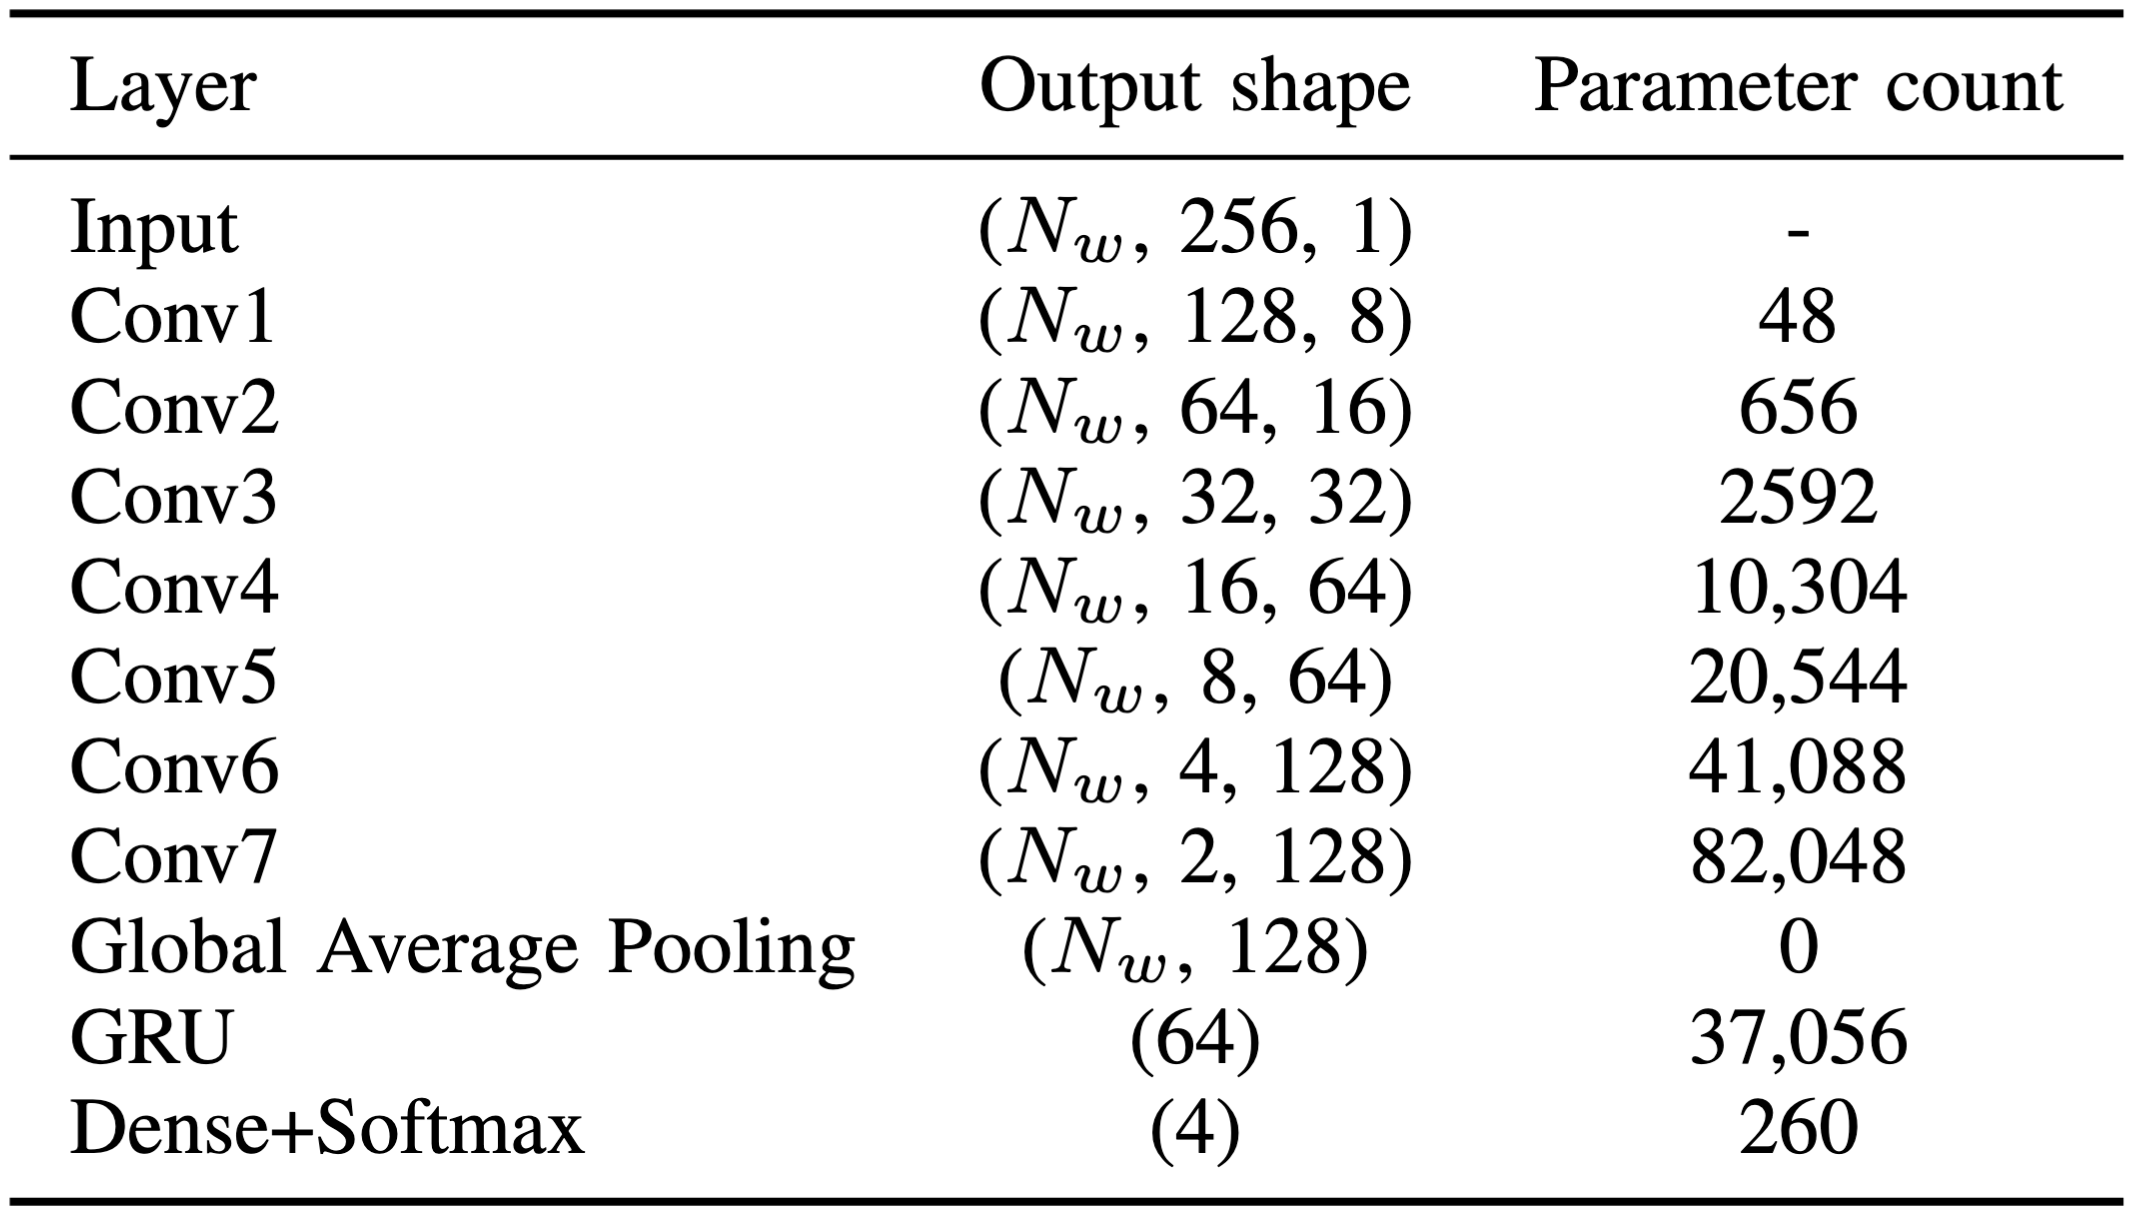
\includegraphics[width=0.7\textwidth]{Graphs/ECG-Paper-Arch.png}
      \caption{Convolutional--recurrent architecture employed by Faraone et al.\ \cite{faraoneConvolutionalRecurrentNeuralNetworks2020}.}
      \label{fig:ecg_paper_arch}
      \end{figure}

      Despite presenting a promising embedded implementation, the approach is subject to several limitations
      that are directly relevant to our work. First, it operates on comparatively short inputs, processing
      windows of only 256 samples and a recurrent sequence of just 128 timesteps, which constrains the
      temporal context available to the model. Second, the recurrent complexity is deliberately curtailed:
      the authors substitute the LSTM of the original architecture with a less expressive GRU specifically
      to reduce the memory footprint and operation count. Finally, and most significantly, the recurrent
      component could not be executed using a general-purpose inference engine; the authors report that
      TensorFlow Lite for Microcontrollers did not support recurrent operators at the time, necessitating a
      hand-written CMSIS-NN implementation.

      A second representative study is the work of Kim et al.\ \cite{kimTinyMLBasedClassificationECG2023},
      which develops a TinyML-based classifier for an ECG monitoring embedded system (TinyCES). In contrast
      to the preceding work, the authors adopt a purely convolutional--fully-connected architecture for the
      binary classification of normal and abnormal ECG segments, comprising two convolutional layers (with
      8 and 16 filters of size $4{\times}1$, respectively), each followed by max-pooling and dropout, and
      terminating in two dense layers.

      The model is implemented using TensorFlow Lite for Microcontrollers and deployed on an Arduino Nano 33
      Bluetooth Low Energy (BLE) Sense board, also based on an ARM Cortex-M4 core. Operating on an input
      window of 180 samples, the converted model occupies a footprint of only 27\,KB and achieves a
      detection accuracy of approximately 97\%.

      \begin{figure}[H]
      \centering
      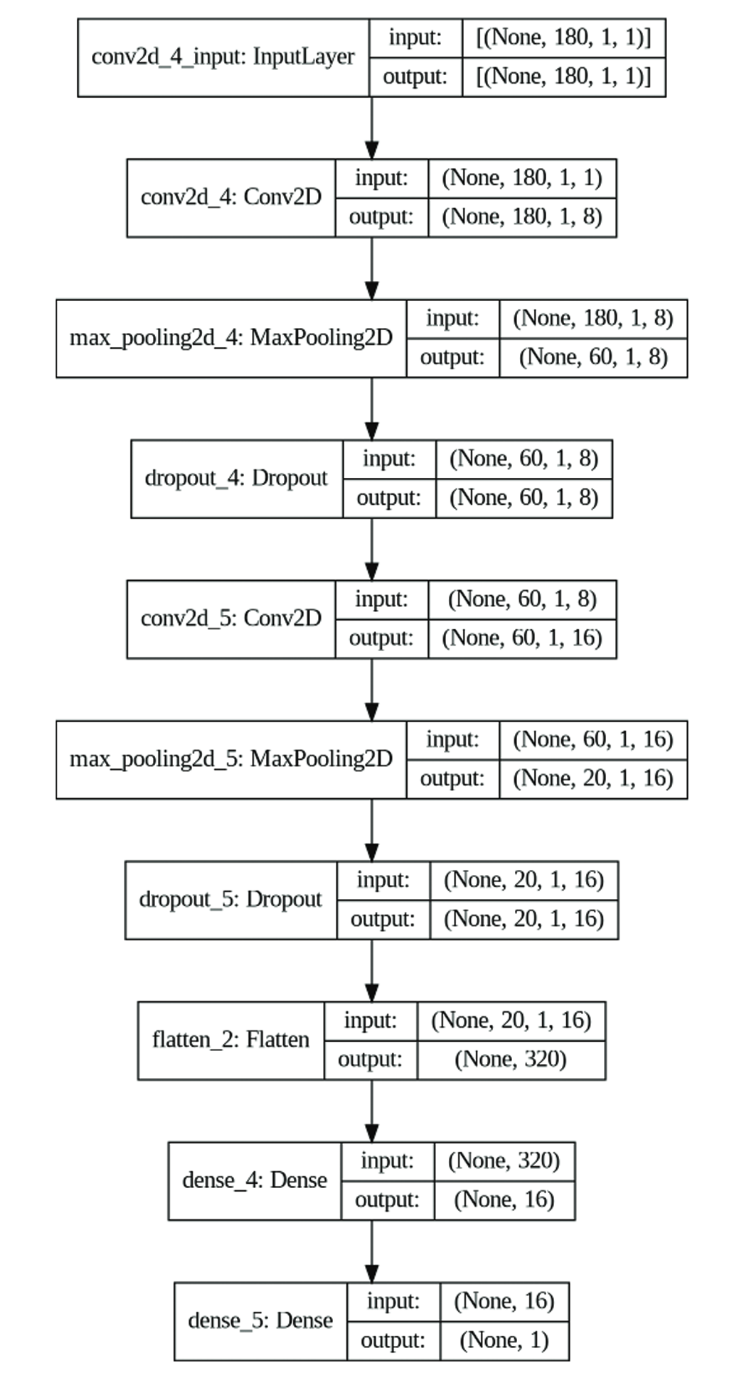
\includegraphics[width=0.7\textwidth]{Graphs/ECG-Monitor-Kim-Paper-Arch.png}
      \caption{Convolutional--fully-connected architecture employed by Kim et al.\ \cite{kimTinyMLBasedClassificationECG2023}.}
      \label{fig:ecg_kim_paper_arch}
      \end{figure}

      The principal limitation of this study lies in the simplicity of its architecture relative to the
      demands of continuous biosignal regression. The model contains no recurrent component whatsoever,
      relying solely on convolutional feature extraction followed by dense classification, and it therefore
      forgoes any explicit modelling of temporal dependencies across the signal. Furthermore, the
      comparatively small input window of 180 samples and the reduction of the task to binary
      classification yield a markedly smaller and less complex model than is required for the multi-channel,
      multi-output gesture regression addressed in this thesis. Consequently, while the work convincingly
      demonstrates the feasibility of fully on-device ECG classification, it does not confront the memory
      and latency challenges posed by recurrent architectures on resource-constrained MCUs.


      \subsection{EMG Signal Processing}

      The closest prior work to this thesis is a pair of studies conducted by the same group at the
      University of Bologna, which together address the complete sEMG processing pipeline---from model design
      through to embedded implementation---on a multicore IoT processor. The first study targets hand-movement
      \emph{classification} \cite{zanghieriRobustRealTimeEmbedded2020}, while the second generalises the same
      methodology to continuous \emph{regression} of hand kinematics \cite{zanghieriSEMGbasedRegressionHand2021}.
      As this thesis is concerned specifically with the implementation side of an analogous pipeline
      these works constitute the principal point of comparison.

      In the classification study \cite{zanghieriRobustRealTimeEmbedded2020}, the authors deploy TEMPONet, a
      dilated Temporal Convolutional Network (TCN), on the 8-core GAP8 processor. The architecture stacks three
      convolutional blocks, each comprising two dilated causal convolutions of kernel size $3{\times}1$ (with full
      padding and increasing dilation) followed by a strided convolution of kernel size $5{\times}1$ and an average
      pooling layer; the convolutional stage is terminated by two fully connected layers with dropout and a SoftMax
      operation. All layers employ ReLU activations and Batch Normalisation
      \cite{zanghieriRobustRealTimeEmbedded2020}. The model is benchmarked on the multi-session NinaPro DB6 dataset,
      operating on short 150\,ms input windows in keeping with the 300\,ms real-time consensus for hand control.

      On the implementation side, the PyTorch model is deployed using the dedicated PULP-NN kernel libraries, which
      exploit the eight RISC-V cluster cores of the GAP8 together with their SIMD extensions. Since the GAP8 lacks a
      floating-point unit, inference is carried out entirely in 8-bit fixed-point arithmetic. To accommodate the
      tight on-chip memory, an automated tiling tool (DORY) partitions the weights and feature maps of each layer
      into tiles that fit the 64\,kB L1 scratchpad and inserts double-buffered DMA transfers between the 512\,kB L2
      memory and L1 so that data movement overlaps with computation \cite{zanghieriRobustRealTimeEmbedded2020}.

      The classification model attains an inter-session accuracy of 49.6\% on the full NinaPro DB6 (7.8 percentage
      points above the prior state of the art) and 93.7\% on a 20-session dataset collected by the authors as a
      proxy for the final deployment. Following int8 quantisation, the network occupies a memory footprint of
      460\,kB and executes a single inference in 12.84\,ms on the GAP8 \cite{zanghieriRobustRealTimeEmbedded2020}.

      The companion regression study \cite{zanghieriSEMGbasedRegressionHand2021} retains the same TCN paradigm but
      adapts and further optimises TEMPONet to estimate five continuous degrees of actuation, evaluating it on
      NinaPro DB8 (which includes two trans-radial amputees). Through channel reduction and int8 quantisation, the
      authors reduce the memory footprint to 70.9\,kB and the inference latency to 4.76\,ms on the GAP8, achieving a
      mean absolute error of 6.89\textdegree---marginally below the float32 LSTM baseline of the dataset
      \cite{zanghieriSEMGbasedRegressionHand2021}. Notably, the authors deliberately favour a purely convolutional
      model over recurrent alternatives, citing evidence that TCNs match or exceed the accuracy of LSTMs on sEMG
      sequence modelling while being substantially more amenable to parallelisation and embedded deployment.

      While both studies represent a compelling state of the art, their design choices differ from those of the
      present work in three respects that are directly relevant to our contribution. First, with regard to model
      complexity, both rely on a feature-extraction-only convolutional backbone and explicitly avoid any recurrent
      component; by contrast, the model deployed in this thesis combines spatial and temporal convolutions,
      residual concatenation, batch normalisation and ELU activations, a downsampling stage, a two-layer LSTM, and
      a dedicated regression head. The presence of a genuine recurrent module is significant, as recurrent layers
      are markedly more difficult to deploy on resource-constrained hardware---precisely the implementation
      challenge this thesis addresses. Second, with regard to the hardware platform, both works target the GAP8, an
      8-core parallel processor with ISA extensions purpose-built for embedded neural-network inference, whereas
      this work targets the single-core ESP32-S3, a substantially more constrained but far cheaper and more widely
      available commodity microcontroller. Third, and most consequentially, their deployment depends on a bespoke,
      platform-specific toolchain (PULP-NN kernels with DORY-based tiling) tightly coupled to the GAP8 architecture,
      rather than on a portable, industry-standard inference framework. The present work instead builds upon LiteRT
      with a segmented, mixed-precision model pipeline, trading a degree of raw efficiency for portability and
      reproducibility on commodity hardware.







    
\chapter{Materials and Methods}

  \section{Dataset Description and Preprocessing}
    \subsection{NinaPro DB2 Dataset}
    The Non-Invasive Adaptive Hand Prosthetics (NinaPro) database is the largest
    publicly available multi-modal benchmark assembled to support machine-learning
    research on human, robotic, and myoelectric hand prostheses. The database
    comprises ten datasets totalling more than $180$ data acquisitions from both
    intact subjects and transradial amputees, spanning electromyographic, kinematic,
    inertial, clinical, neurocognitive, and eye--hand coordination modalities. Each
    acquisition is obtained by simultaneously recording surface electromyography
    (sEMG) from the forearm together with the kinematics of the hand and wrist while
    the subject performs a predefined set of movements and
    postures~\cite{atzoriCharacterizationBenchmarkDatabase2015}.

    In this work we employ the second NinaPro database (DB2), which contains
    recordings from $40$ intact subjects performing $49$ distinct gestures, each
    repeated six times. The sEMG signals were acquired using twelve Delsys Trigno
    wireless electrodes, and the corresponding hand kinematics were captured using a
    CyberGlove~II data glove; the dataset additionally provides inertial and force
    modalities. For each recording, DB2 supplies twelve sEMG channels, thirty-six
    accelerometer channels (the three-axis accelerometers integrated into the twelve
    electrodes), and twenty-two glove channels containing the uncalibrated outputs of
    the CyberGlove sensors, which are approximately proportional to the joint angles
    of the hand and wrist.

    \subsubsection{Channel and Gesture Selection}

    To match the input dimensionality of our model and the constraints of the target
    hardware, we restrict the data to a subset of channels and gestures. Of the twelve
    available sEMG channels, we retain only the first eight, which correspond to
    electrodes equally spaced around the forearm at the level of the radio-humeral
    joint. On the output side, the regression target is reduced to two glove channels,
    selected to capture the degrees of freedom most relevant to the gestures under
    study: one channel associated with finger abduction and fist closure, and one
    associated with wrist extension and flexion. For each gesture, the glove channel
    that is not actuated by that movement is set to zero, so that the model is trained
    to predict only the degree of freedom genuinely exercised by the gesture.

    From the full set of $49$ gestures we select five: abduction of all fingers,
    fingers flexed together into a fist, wrist flexion, wrist extension, and wrist
    extension with a closed hand; the remaining gestures are discarded. This yields a
    focused regression task over a small, well-characterized set of movements suited
    to deployment on a resource-constrained device.

  \subsubsection{Preprocessing}

  Each trial is band-pass filtered using a fourth-order Butterworth filter with a
  passband of $5$--$450$~Hz, attenuating frequency components outside this range. 
  Every trial is epoched to a fixed length of five seconds, corresponding to $10{,}000$
  samples at the DB2 sampling rate. The epoched recordings are then segmented into
  non-overlapping windows; that is, the windowing hop is set equal to the window
  length, so that consecutive windows tile each trial without overlap. The window
  length itself is treated as an experimental parameter, allowing its effect on both
  predictive accuracy and on-device latency to be studied systematically.

  \section{Deep Learning Model Architecture}

  The model architecture used in this work was developed by Koellner et al.\ at the
  Institute for Signal Processing and System Theory, University of Stuttgart, and
  was trained on the NinaPro DB2 dataset. It is a fully convolutional--recurrent
  regression network that maps a windowed, multi-channel sEMG input of shape
  $(B, C, T)$---where $B$ is the batch size, $C$ the number of input channels, and
  $T$ the window length---to a continuous estimate $\hat{y}$. For the present study,
  the input comprises $C = 8$ EMG channels. The network is organized into four
  functional stages: a convolutional feature extractor (input block), a
  convolutional downsampling block, a recurrent block, and a regression head, as
  illustrated in Figure~\ref{fig:model_arch}.

  \paragraph{Input block (feature extraction).}
  The input block performs feature learning along the temporal and spatial
  (inter-channel) axes in sequence. The windowed signal is first expanded to
  $(B, 1, C, T)$ and passed through a temporal two-dimensional convolution with
  $48$ output channels, a kernel of size $(1, k)$ and same padding, followed by
  batch normalization. A spatial convolution with a kernel of size $(C, 1)$ and
  channel-wise grouping then mixes information across the input channels, after
  which the tensor is squeezed back to $(B, 48, T)$ and subjected to a further batch
  normalization, an ELU activation, and dropout with a rate of $0.5$. The output of
  the input block is concatenated with the original input along the channel
  dimension, yielding a feature representation of shape $(B, 48 + C, T)$. This
  concatenation acts as a residual-style skip connection that preserves the raw
  input alongside the learned features.

  \paragraph{Downsampling block.}
  The concatenated feature map is downsampled along the temporal axis by a strided,
  grouped one-dimensional convolution with $48 + C$ output channels, a kernel of
  size $9$, same padding, and a stride equal to the downsampling factor of $2$. This
  is followed by batch normalization, an ELU activation, and dropout with a rate of
  $0.5$, producing a tensor of shape $(B, 48 + C, T/2)$ in which the temporal
  resolution has been halved.

  \paragraph{Recurrent block.}
  Temporal dependencies are modelled by a two-layer unidirectional LSTM with a
  hidden size of $48 + C = 56$, which preserves the channel dimension of its input
  and outputs a sequence of shape $(B, 48 + C, T/2)$.

  \paragraph{Regression head.}
  The final stage is a fully connected regressor that maps the LSTM output to the
  target. It consists of a linear layer projecting from $48 + C$ to a hidden width
  of $11$, a $\tanh$ activation, and a second linear layer projecting from $11$ to
  the $C$ output dimensions, yielding the prediction $\hat{y}$ of shape
  $(B, C, T/2)$.

  \subsubsection{Model Configurations}

  The architecture is highly configurable. To investigate the effect of the
  receptive field of the temporal convolution on both accuracy and on-device
  performance, we evaluated two configurations that differ principally in the
  dilation and kernel size of the input block and in the depth of the regression
  head; all remaining hyperparameters are held constant. Both configurations use a
  dropout rate of $0.5$ throughout, a downsampling stride of $2$, and a two-layer
  LSTM with a hidden size of $56$.

  Model~A\footnote{Designate as baseline / dilated as appropriate.} employs an
  undilated temporal convolution with a wide kernel: the input block uses a kernel
  size of $51$, $48$ output channels, and a dilation of $1$, and the regression head
  comprises four layers. Model~B instead employs a dilated temporal convolution with
  a narrower kernel: the input block uses a kernel size of $17$, $48$ output
  channels, and a dilation of $3$, with a three-layer regression head. The
  configurations are summarized in Table~\ref{tab:model_configs}.

  \begin{table}[htbp]
    \centering
    \caption{Hyperparameter configurations of the two evaluated models.}
    \label{tab:model_configs}
    \small
    \begin{tabular}{llcc}
      \toprule
      Block & Hyperparameter & Model~A & Model~B \\
      \midrule
      \multirow{4}{*}{Input}
        & Output channels & 48 & 48 \\
        & Kernel size     & 51 & 17 \\
        & Dilation        & 1  & 3  \\
        & Dropout         & 0.5 & 0.5 \\
      \midrule
      \multirow{3}{*}{Downsample}
        & Kernel size & 9 & 9 \\
        & Stride      & 2 & 2 \\
        & Dropout     & 0.5 & 0.5 \\
      \midrule
      \multirow{2}{*}{LSTM}
        & Layers       & 2  & 2  \\
        & Hidden size  & 56 & 56 \\
      \midrule
      Regressor & Layers & 4 & 3 \\
      \bottomrule
    \end{tabular}
  \end{table}
      \begin{figure}[H]
        \centering
        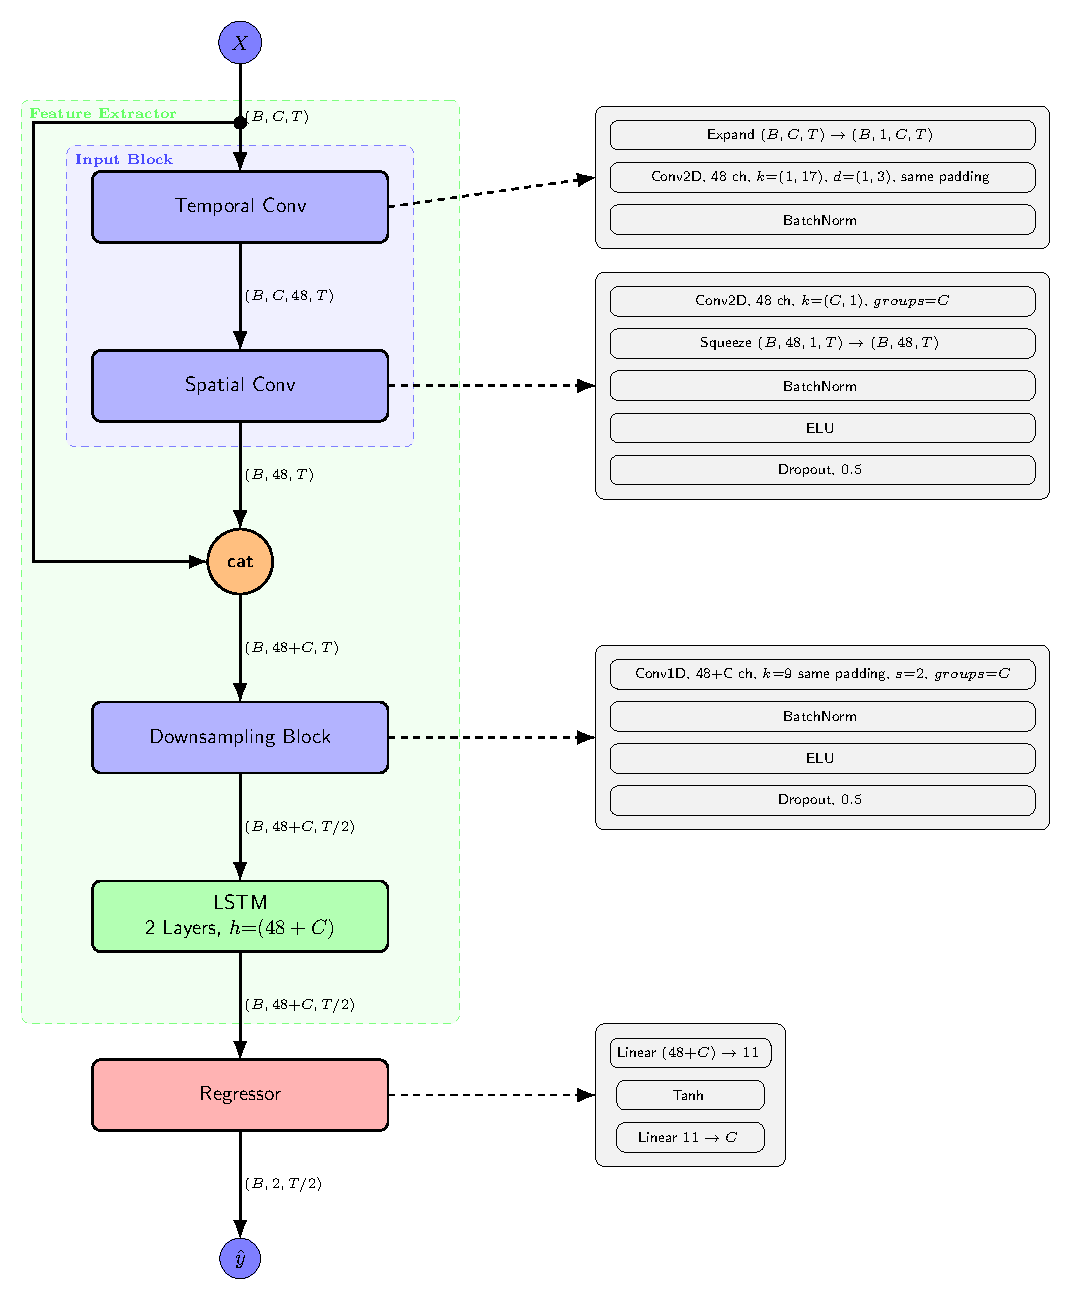
\includegraphics[width=0.8\textwidth]{Model.pdf}
        \caption{Deep Learning Architecture used for EMG regression by Koellner et al}
        \label{fig:model_arch}
      \end{figure}
  \section{Hardware}
    \subsection{ESP32-S3 Specifications}

    All experiments in this work were conducted on an ESP32-S3-based development
    board (ESP32-S3 UNO) equipped with $16$~MB of external flash and $8$~MB of
    external PSRAM (pseudo-static RAM). The ESP32-S3 was selected because it is one
    of the few low-cost microcontrollers whose architecture incorporates dedicated
    hardware acceleration for the integer arithmetic that dominates quantized
    neural-network inference. This subsection summarizes the characteristics of the
    platform that are most relevant to on-device machine learning and to the
    single-instruction-multiple-data (SIMD) execution exploited by the ESP-NN
    backend. All figures are taken from the official \textit{ESP32-S3 Technical
    Reference Manual} \cite{espressif-esp32-s3-TRM}.

    \subsubsection{Processor and Memory Architecture}

    The ESP32-S3 is a dual-core system built around two Harvard-architecture
    Tensilica Xtensa\textregistered{} LX7 CPUs, each capable of operating at a clock
    frequency of up to $240$~MHz. On-chip memory comprises $384$~KB of internal ROM
    and $512$~KB of internal SRAM, the latter accessible by the CPU typically within
    a single clock cycle. This relatively small fast-memory budget is a defining
    constraint of the platform: the complete set of model parameters, the
    interpreter's tensor arena, and all runtime buffers must either fit within the
    internal SRAM or be placed in the slower external memory.

    To accommodate larger models, the ESP32-S3 supports external flash and external
    RAM through its SPI interfaces (including the Octal SPI and OPI modes used by
    high-bandwidth PSRAM), addressing up to $1$~GB of each. The CPU does not access
    external memory directly; instead, the external address space is mapped into the
    CPU address space through a cache. Up to $32$~MB of the data-bus address space can
    be mapped to external RAM in individual $64$~KB blocks. This indirection is
    significant for inference latency: data resident in the $8$~MB PSRAM of our board
    is reached through the cache rather than at SRAM speed, so any working set
    (notably a large activation arena) that spills out of internal SRAM into PSRAM
    incurs additional access latency on cache misses.

    Memory access on the ESP32-S3 is mediated by a dual-core-shared instruction cache
    (ICache) and data cache (DCache). The ICache can be configured to $16$~KB or
    $32$~KB with a block size of $16$~B or $32$~B, while the DCache can be configured
    to $32$~KB or $64$~KB with a block size of $16$~B, $32$~B, or $64$~B. The cache
    controller fetches from external memory on a miss and supports write-back, clean,
    invalidate, and preload operations. Because cache misses against PSRAM are far
    more expensive than internal-SRAM accesses, the locality of the inference working
    set has a direct effect on measured latency---a consideration that motivates
    keeping the tensor arena small enough to remain in internal memory wherever
    possible.

    \subsubsection{Processor Instruction Extensions (PIE) and SIMD}

    The feature most relevant to this work is the ESP32-S3's Processor Instruction
    Extensions (PIE), a vector instruction set defined through the Tensilica
    Instruction Extension (TIE) language and added specifically to accelerate AI and
    digital-signal-processing workloads. The PIE follows the SIMD paradigm, applying a
    single instruction across multiple data elements packed into wide vector
    registers, and supports $8$-bit, $16$-bit, and $32$-bit integer vector operations.

    The unit provides a bank of eight $128$-bit general-purpose vector registers
    (denoted QR). Each register can be interpreted as sixteen $8$-bit, eight $16$-bit,
    or four $32$-bit lanes, depending on the operation. The arithmetic logic unit
    contains sixteen $8$-bit multipliers and eight $16$-bit multipliers, enabling up
    to sixteen multiply-and-accumulate operations to be issued in a single $8$-bit
    instruction. Results accumulate into dedicated wide registers---a pair of
    $160$-bit accumulators (QACC\_H and QACC\_L) and a $40$-bit accumulator
    (ACCX)---which preserve the precision of summed integer products before the result
    is requantized and written back. Arithmetic instructions such as multiplication,
    shifting, and accumulation can transfer data while computing, and the extension
    supports saturating arithmetic and non-aligned $128$-bit vector loads.

    This hardware is directly responsible for the performance characteristics reported
    in Chapter~\ref{ch:results}. The wide multiply-accumulate datapath maps naturally
    onto the dominant operations of the inference pipeline---the matrix
    multiplications underlying the fully connected and LSTM layers, and the
    convolutions of the feature-extraction stages---but only when those operations are
    expressed as $8$-bit integer arithmetic. The eight $8$-bit lanes per multiplier
    group and the abundance of $8$-bit multipliers explain why the ESP-NN kernels are
    optimized exclusively for \texttt{int8} operands on this platform, and why the
    floating-point execution paths, which cannot use the PIE multiply-accumulate
    units in the same way, are substantially slower. The architectural details
    presented here therefore underpin the large \texttt{int8}-versus-floating-point
    latency gap observed in our measurements.

  
  \section{Quantization}
  Normally, Deep learning pipelines rely on floating point operations and embed their parameters (i.e weights and biases)
  as float32s. Unfortunately, not all MCU architectures have embedded FPU (floating point units) to handle calculations
  in floating point notations. In addition, chips that have dedicated FPUs in their architecture, for handling float32
  data, suffer from longer processing times and resource intensive operation compared to the faster integer arithmetic
  units \cite{krishnamoorthiQuantizingDeepConvolutional2018,jacobQuantizationTrainingNeural2017,nagelWhitePaperNeural2021}.Furthermore, floating point numbers necessitate
  larger spaces in memory for tensor allocations (i.e inputs, outputs, model parameters and activations)
  \cite{krishnamoorthiQuantizingDeepConvolutional2018}.
  \\
  For these reasons, different quantization schemes are widely adopted across TinyML literature It is also the case on many MCU platforms (like the ESP32 and ESP32s3),
  that optimized low-level kernels for ML ops (like Convolutions and MatMuls) are exclusively written with quantization schemes, like INT8, in mind.
  In fact, 8-bit quantization has been shown to reduce model sizes by a factor of 4 and produce a speedup gain of 2x-3x ,even 
  10x on specialized processors, compared to float Implementations\cite{krishnamoorthiQuantizingDeepConvolutional2018}.

  On the other hand, quantization algorithms are not lossless since they map a continuous floating point representation into a discrete
  range. A degradation in final accuracy is always expected in quantized outputs. That's why quantization pipelines require careful fine-tuning to balance
  quality and performance.  
  \subsection{Quantization Types and Schemes}
  Quantization schemes have been categorized into many section. In this work, we are going to outline schemes that are only relevant to TinyML research.
  
  \subsubsection{Data Types}
  By default, popular frameworks like PyTorch, Tensorflow and JAX utilize single-precision floating point numbers (float32s).
  Quantization schemes can then be categorized into the output data types that these float32s are converted to. 
  \\\\
  \textbf{Float16} quantization uses half the space used by float32s while maintaining the floating point interface as float32s.
  However, float16 adoption in MCU architectures still remain rare. Most MCUs don't have dedicated kernels for handling float16s and just
  use float32 interfaces rendering float16 optimizations completely useless. Others are unable to handle float16 data and immediately throw exceptions.
  \\\\
  \textbf{Int8, Int16, Int32} quantization are by far the most used. Most MCU architectures are optimized for handling integer operations which 
  makes int quantization adoption easier and more natural. Low-Level kernels usually use a mix of various integer sizes in their internal Implementation,
  usually inputs, outputs and weights are int8 while biases use larger formats like int32s. 

  \subsubsection{Asymmetric vs symmetric quantization}
  \textbf{symmetric} quantization restricts the zero-point to 0. It only computes the scale of the floating-point values 
  as the ration between the absolute maximum value in the floating point range and the maximum value in the quantization
  range. Commonly used for quantizing weights and biases as\cite{krishnamoorthiQuantizingDeepConvolutional2018}. The
  reason why it is preferred for weights is because using asymmetric quantization (with an additional zero-point value
  for weights) adds an additional term to each \textbf{W . x} calculation which costs additional compute time during inference
  \cite{nagelWhitePaperNeural2021}.

  \begin{equation}
  \begin{aligned}
      x_{int} &= \operatorname{round}\!\left(\frac{x}{\Delta}\right) \\
      x_{Q} &= \operatorname{clamp}\!\left(-N_{levels}/2,\; N_{levels}/2 - 1,\; x_{int}\right) && \text{if signed} \\
      x_{Q} &= \operatorname{clamp}\!\left(0,\; N_{levels} - 1,\; x_{int}\right) && \text{if un-signed} \\
      x_{out} &= x_{Q}\,\Delta && \text{(de-quantization)}
  \end{aligned}
  \end{equation}

  \textbf{Asymmetric} quantization calculates an optimal new zero-point value to map the floating point zero to it. Preferred for activations.
  \subsubsection{Quantization Aware Training (QAT) vs Post Training Quantization (PTQ)}
  
  \begin{equation}
  \begin{aligned}
      x_{int} &= \operatorname{round}\!\left(\frac{x}{\Delta}\right) + z \\
      x_{Q} &= \operatorname{clamp}\!\left(0,\; N_{levels} - 1,\; x_{int}\right) \\
      x_{float} &= (x_{Q} - z)\,\Delta && \text{(de-quantization)}
  \end{aligned}
  \end{equation}

  \textbf{Post Training Quantization (PTQ)} works on quantization pre-trained DL models, trained using default floating-point numbers.
  The quantizing algorithm takes pre-trained weights and biases and calculates the appropriate scaling and shifting parameters. For activations,
  it uses a representative dataset (representing a sample of input values in floating space) and propagates it through the model to get a closer 
  statistical model of how values fluctuate in the actual model in order to map it to the quantized range. PTQs are widely adopted in pipelines 
  that aim at deploying normal, pre-trained models, usually not co-designed for TinyML use, on Edge device without having to re-train the model
  \cite{krishnamoorthiQuantizingDeepConvolutional2018,nagelWhitePaperNeural2021}.
  \\\\
  \textbf{Quantization Aware Training (QAT)} involves having quantization in mind
  during the training of the actual model, with simulated quantization applied at every
  step of gradient descent so that the model learns to compensate for quantization noise.
  The weights are maintained in floating point and updated using floating-point gradients,
  while a simulated quantization operation (fake quantization) emulates the effect of
  integer inference during the forward and backward passes. While this method can provide
  higher accuracies than PTQ \cite{krishnamoorthiQuantizingDeepConvolutional2018,nagelWhitePaperNeural2021}, it
  necessitates active co-design of the DL model and is not viable for quantizing all
  available models, since it requires retraining in the presence of simulated quantization,
  which demands additional training resources and time-consuming retraining.

  \begin{equation}
  \begin{aligned}
      w_{float} &= w_{float} - \eta\,\frac{\partial L}{\partial w_{out}}\cdot I_{w_{out}\in(w_{min},\,w_{max})} \\
      w_{out} &= \operatorname{SimQuant}(w_{float})
  \end{aligned}
  \end{equation}
  
  \subsubsection{Hybrid vs Full quantization}
  \textbf{Hybrid} quantization is defined as quantizing the inputs, weights and biases only while leaving intermediate activations
  as floating point. While this can improve final accuracy since a full quantization is not adopted and activations remain in their full floating point
  resolution, many MCU platforms and frameworks do not fully support mixed precision computation. In addition, Hybrid models produced the overhead of having
  to requantize activations after each neural layer which can detrimentally impact the final inference time and the needed allocation space for larger float32 intermediate
  values.
  \\\\
  \textbf{Full} quantization involves the quantization of the entire Pipeline eliminating the need for intermittent requantization steps and produces more faster
  and more lightweight models since there are not intermediate floats. However, for full quantization, more overhead is needed for calculating additional quantization
  parameters for activation layers and , depending on the quantization scheme used, may require a set of representative data to calculate those quantization parameters.s
  
  \subsubsection{Quantization granularity}
  Quantization can be done with varying degrees of resolution at the cost of producing an increasing amount of quantization parameters and settings.

  \textbf{Per Tensor} quantization involves calculating scaling and shifting params for each tensor involved in the pipeline. 
  This scheme is preferred for activations \cite{krishnamoorthiQuantizingDeepConvolutional2018}.
  \\\\
  \textbf{Per Channel} quantization involves having a set of quantization params per each channel in a tensor. This presents
  a more granular quantization scheme as it accounts for distribution differences between individual channels in the data at hand.
  This is the recommended method for stored weights \cite{krishnamoorthiQuantizingDeepConvolutional2018,nagelWhitePaperNeural2021}.

  \subsection{Quantization Scheme Used}
  In this work, we opted for a PTQ quantization scheme. In order to comply with ESP-NN backend functions, we use full int8 quantization across the 
  entire model with int32 accumulators and int32 for biases as presented here \cite{jacobQuantizationTrainingNeural2017}. Since ESP-NN uses the same quantization schemes as TFlite runtime, 
  we are using per tensor asymmetric quantization for inputs and activations while using symmetric per channels quantization
  for both weights and biases. Similar 8-bit PTQ schemes, with per channel quantization for weights and per layer quantization of activations, have shown
  accuracies within 2 percent of floating point networks, particularly for CNN architectures \cite{krishnamoorthiQuantizingDeepConvolutional2018}. 

\section{Software and Tools}
  \subsection{ESP-NN Library}
  The ESP-NN library contains optimized NN (Neural Network) functions for various Espressif chips. They are the backend used
  by TensorFlow Lite Micro on esp32 chips. It supports ESP32, ESP32-S3, ESP32-P4 and ESP32-C3 chips. While it provides
  generic optimizations for most chips, it provide assembly optimized versions for ML dedicated chips like ESP32-S3.

  The optimized ESP-NN libraries on ESP32-S3 chip are only dedicated for Int8 quantized operations. For matrix multiplications,
  the core arithmetic operations behind fully connected and LSTM layers, 2 functions are available for use.
  \texttt{esp\_nn\_fully\_connected} which is used for per tensor weight quantization and the \texttt{esp\_nn\_fully\_connected\_per\_ch} variant for per channel quantized weights.

  Similar to \cite{jacobQuantizationTrainingNeural2017}, ESP-NN uses int32 accumulators for accumulating the intermediate products in matmul operations.
  This follows directly from the integer-arithmetic-only formulation of \cite{jacobQuantizationTrainingNeural2017}, where each real value $r$ is represented
  through an affine mapping $r = S(q - Z)$ from its quantized integer $q$, with scale $S$ and zero-point $Z$. Under this mapping, a quantized matrix product
  reduces to:
  \begin{equation}
    q_3^{(i,k)} = Z_3 + M \sum_{j=1}^{N} \left(q_1^{(i,j)} - Z_1\right)\left(q_2^{(j,k)} - Z_2\right),
  \end{equation}
  where the summation is performed entirely in integers and held in a wide (int32) accumulator, exactly as ESP-NN does. The only non-integer term is the
  multiplier $M = S_1 S_2 / S_3$, which depends only on the fixed tensor scales and is therefore constant at inference. Since $M \in (0,1)$, it is expressed
  in the fixed-point form $M = 2^{-n} M_0$ with $M_0 \in [0.5, 1)$. This is precisely how the rescaling is discretized into the kernel's two integer parameters:
  $M_0$ becomes the fixed-point multiplier \texttt{out\_mult}, and the factor $2^{-n}$ becomes a rounding right-shift by \texttt{out\_shift}. Requantization thus
  reduces to one integer multiply followed by a shift, keeping the matmul pipeline entirely integer-only.
  
  \subsection{LiteRT (TensorFlow Lite) Framework}

  LiteRT is the successor to the widely adopted TensorFlow Lite pipeline. Developed
  by Google, TensorFlow Lite was designed to streamline TinyML workflows by
  providing a means of converting pre-trained TensorFlow models into a flatbuffer
  representation (the \texttt{.tflite} format). This flatbuffer is subsequently read
  by the TensorFlow Lite Micro interpreter on the target device to perform
  inference. A principal strength of the framework is that it delegates execution to
  the optimized neural-network kernels native to the host microcontroller---such as
  ESP-NN for Espressif devices and CMSIS-NN for ARM-based devices---thereby
  achieving near-native performance without requiring the developer to implement the
  model from scratch using low-level kernels.

  The underlying development pipeline of TensorFlow Lite Micro (TFLM) comprises two
  distinct stages, namely an offline conversion stage performed on a host machine and
  an on-device inference stage executed on the target microcontroller
  \cite{davidTensorFlowLiteMicro2021}. In the offline stage, a model trained within
  the TensorFlow environment is processed by the TensorFlow Lite converter, which
  applies optimisations such as quantisation and the folding of constant expressions
  (e.g.\ batch normalisation) before serialising the result into a portable FlatBuffer
  file (\texttt{.tflite}). The FlatBuffer format is well suited to embedded targets, as
  its memory-mapped representation requires no unpacking at run time and can be readily
  embedded into the application binary as a C source array, obviating the need for a
  file system on devices that lack one \cite{davidTensorFlowLiteMicro2021}.

  In the on-device stage, rather than generating native code from the model, TFLM
  adopts an interpreter-based design in which a single, static body of execution code
  reads the FlatBuffer at run time to determine which operators to invoke and from
  where to draw their parameters \cite{davidTensorFlowLiteMicro2021}. This approach
  favours portability and field-updatability over the marginal performance gains of
  code generation, and incurs negligible overhead in practice, since the long-running
  neural-network kernels dominate execution time and amortise the cost of
  interpretation \cite{davidTensorFlowLiteMicro2021}. At initialisation, the application
  supplies the interpreter with the model, an operator resolver (\texttt{OpResolver})
  that maps the operators present in the model to their implementations whilst
  minimising binary size, and a contiguous, fixed-size memory region termed the
  \emph{arena}. The interpreter plans and allocates all required buffers from this arena
  during the initialisation phase and performs no further dynamic allocation during
  inference, thereby avoiding the heap fragmentation that would otherwise jeopardise
  long-running embedded applications \cite{davidTensorFlowLiteMicro2021}. It is precisely
  at the operator level of this interpreter that the aforementioned vendor-optimised
  kernel libraries are substituted for the portable reference implementations, allowing
  hardware-specific acceleration without modification to the surrounding framework
  \cite{davidTensorFlowLiteMicro2021}.

  The principal limitation of TensorFlow Lite was its tight coupling to the
  TensorFlow ecosystem, which required PyTorch models to be translated into
  TensorFlow before conversion. This translation was not straightforward: it
  entailed first exporting the PyTorch model to the ONNX interchange format and then
  converting the ONNX model to TensorFlow. In our experience, this multi-stage
  pipeline incurred substantial conversion overhead and, in many cases, failed to
  complete owing to discrepancies between the PyTorch and TensorFlow model
  representations---for example, differences in tensor memory layout (NCHW versus
  NHWC) and in the expected index of the batch dimension when exporting LSTM layers.

  Released in 2024, LiteRT removes this dependency on the TensorFlow ecosystem,
  repositioning the framework as a cross-framework solution that no longer requires
  intermediate conversion formats, while retaining the \texttt{.tflite} file format
  for backward compatibility. LiteRT additionally exposes a range of configurable
  quantization schemes, including Float16, hybrid, and full Int8 quantization.

  \subsubsection{Modular Architecture}

  To address these issues, we adopted a modular deployment strategy. Rather than
  exporting the entire network as a single flatbuffer with one long and costly graph,
  we partitioned the model at carefully chosen points so as to eliminate redundant
  operations and to permit independent selection of quantization scheme and numerical
  precision for each part, with the joint objectives of minimizing mean squared error
  and reducing the memory footprint. After experimenting with the placement of these
  partitions, we settled on three split points that divide the model into four stages.

  The partitioning was performed non-destructively: each stage was reconstructed as a
  standalone model from the trained network, with the corresponding parameters copied
  into the appropriate stage. The resulting four stages comprise two convolutional
  models for the feature-extraction operations (the temporal and spatial convolutions
  of the input block forming the first stage, and the downsampling convolution forming
  the second), a single instance of the two-layer LSTM cell as the third stage, and
  the regression head as the fourth.

  A key element of this strategy concerns the export of the recurrent stage. Rather
  than unrolling and exporting the LSTM over the entire window---which had produced
  the prohibitive footprint and initialization cost described above---the LSTM is
  exported as a single block spanning only a small, fixed number of timesteps (one or
  five in our experiments) and is then invoked repeatedly within a loop on the device,
  together with the regression head, to process the full sequence. Because only one
  short LSTM block resides in memory at any time and is reused across iterations,
  rather than the complete set of unrolled timesteps being materialized as distinct
  cells, this windowed export reduces the memory overhead of the recurrent stage
  considerably. The number of timesteps processed per block (the LSTM block step size)
  therefore becomes a deployment parameter that trades recurrent loop overhead against
  the working memory of the stage. Taken together, these measures reduced the memory
  footprint from over $1.5$~MB to approximately $260$~KB for the complete model.
  Crucially, the modular decomposition also enabled mixed-precision deployment,
  allowing accurate floating-point LSTM stages to operate alongside optimized
  Int8-quantized convolutional stages.

  \subsubsection{Graph-Level Transformations for Quantization}

  Two further non-destructive transformations of the model graph were necessary to
  obtain correct and efficient quantized stages.

  First, the batch-normalization layers were folded manually into the weights of the
  preceding convolutions. The LiteRT converter was unable to fuse the
  \texttt{BatchNorm1d} layers on its own; instead, it realized each normalization as a
  separate pair of multiply and add operations in the graph. Beyond the redundant
  computation this introduced, it aggravated the quantization problem, since both
  operations were placed inside a floating-point quantize/dequantize island. We
  therefore folded the batch-normalization parameters back into the corresponding
  convolution weights and biases analytically and removed the layers from the graph,
  eliminating both the spurious operations and the associated precision conversions.

  Second, the one-dimensional convolutions were reformulated as two-dimensional
  convolutions. The LiteRT and TensorFlow Lite Micro toolchain does not quantize
  \texttt{Conv1D} operations by default; expressing the same computation as a
  \texttt{Conv2D} with a singleton spatial dimension was required for the
  convolutional stages to be quantized correctly.

  \subsubsection{Experimental Workflow}

  The experimental workflow proceeds as follows. A configuration-driven system accepts
  a list of model configurations---specifying parameters such as the window length and
  the LSTM block step size---and batch-converts each configuration to the LiteRT
  format, exporting eight models per configuration: four in floating point and four
  Int8-quantized, corresponding to the four pipeline stages. The exported models are
  then packed into a single contiguous binary file and flashed to a dedicated partition
  of the microcontroller's flash memory. The complete input trial is exported alongside
  it, together with the reference output produced by the original PyTorch model, against
  which the mean squared error is computed. On the ESP32-S3, a continuous loop iterates
  over all configurations to generate the final results.


  
  \chapter{Results}
  \section{Comparison of ML Ops Performance on the ESP32-S3 using Random Weights under different Quantization Schemes}
  In order to evaluate general Model perfromance on the esp32s3, we had to create our own small benchmark to evaluate
  the behavior of different data layers and how they react to different parameter changes and to int8 quantization used.

    \begin{figure}[H]
      \centering % Centers the image horizontally
      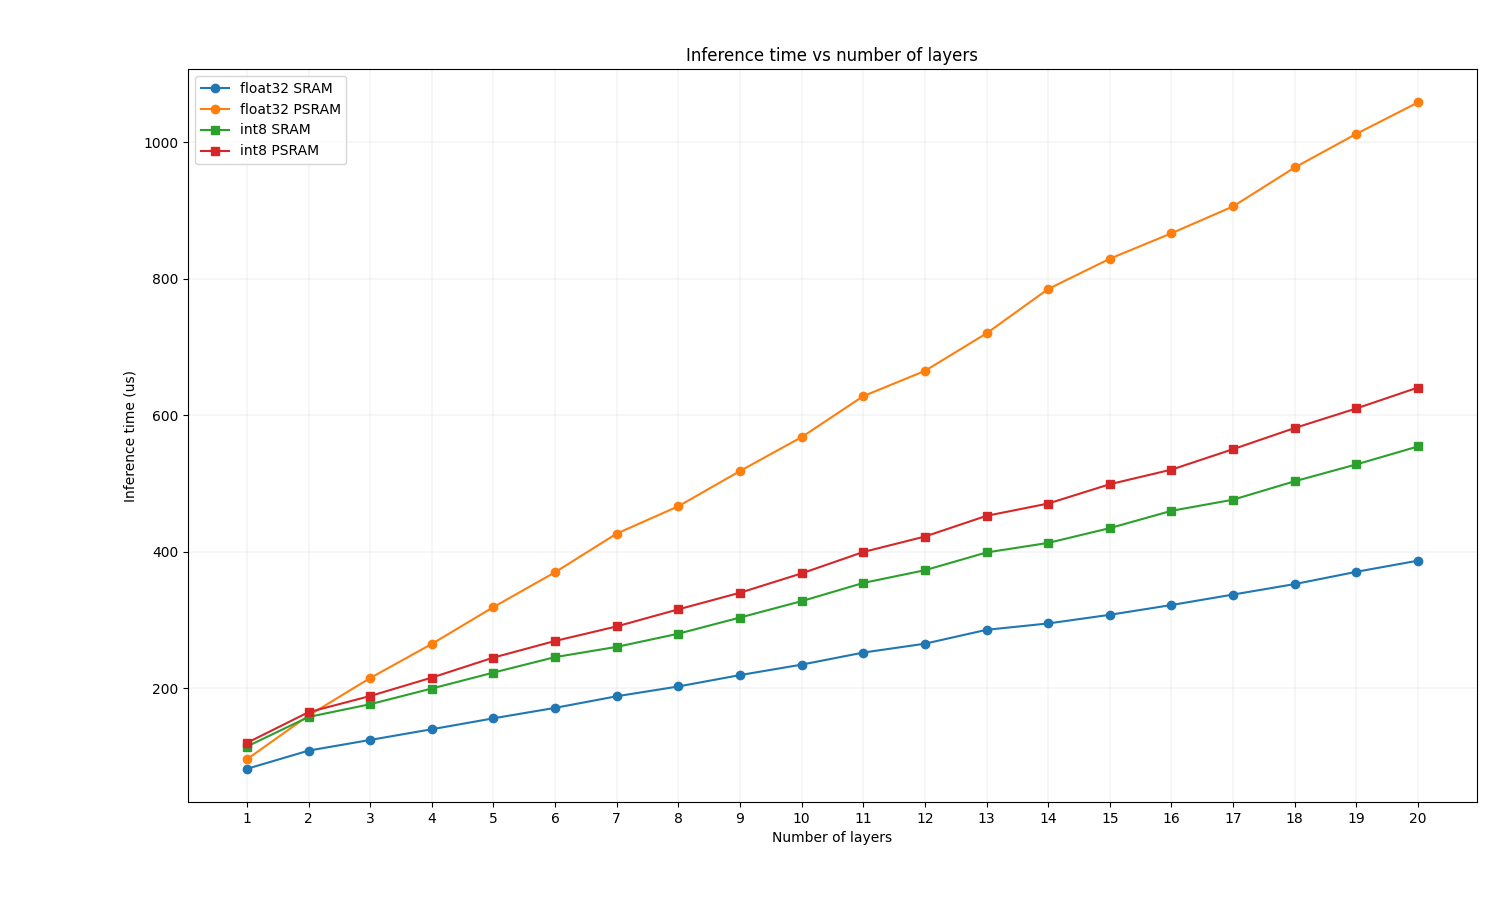
\includegraphics[width=0.7\textwidth]{Graphs/Dense-Layer-Inference.png} % Omit the file extension
      \caption{Figure shows latency of dense layers against the amount of layers used 
      in a geometric decay.}
      \label{fig:dense_layers_latency}
    \end{figure}

    The above graph shows how the number of layers impacts the final latency for dense
    layers, where a geometric falloff determines the number of units at each stage,
    decaying from $50$ down to $2$. Across all four configurations latency grows
    approximately linearly with the number of layers. The effect of int8 quantization,
    however, depends strongly on the memory in which the model resides. On PSRAM, int8
    quantization reduces latency relative to float32 (e.g.\ $\sim\!640\,\mu s$ vs.\
    $\sim\!1060\,\mu s$ at $20$ layers), as the four-fold reduction in weight size lowers
    traffic over the slow external bus on this memory-bound workload. On SRAM the trend
    reverses: int8 is consistently slower than float32 (e.g.\ $\sim\!555\,\mu s$ vs.\
    $\sim\!386\,\mu s$ at $20$ layers), because the workload becomes compute-bound and the
    ESP32-S3's hardware floating-point unit executes each float multiply-accumulate in a
    single instruction, whereas the int8 path incurs additional per-channel requantization
    overhead. The fastest configuration overall is float32 on SRAM, and the slowest is
    float32 on PSRAM.

    \begin{table}[htbp]
      \centering
      \caption{Conv2D layers performance on the ESP32-S3.}
      \label{tab:conv_timing}
      \small
      \fittable{tables/conv_timing.tex}
    \end{table}

    \begin{table}[htbp]
      \centering
      \caption{Conv2D layers performance on the ESP32-S3.}
      \label{tab:conv_memory}
      \small
      \fittable{tables/conv_memory.tex}
    \end{table}

    \begin{figure}[H]
      \centering % Centers the image horizontally
      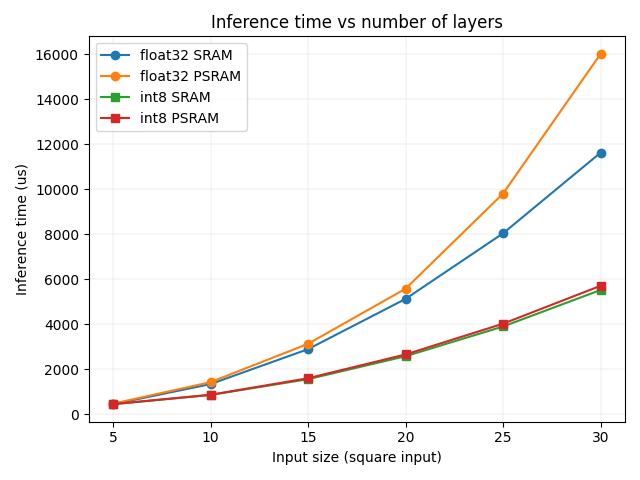
\includegraphics[width=0.7\textwidth]{Graphs/Conv2D-input-size-inference.png} % Omit the file extension
      \caption{Figure shows latency of Conv2D layers against Input Size.}
      \label{fig:conv2D_input_size}
    \end{figure}

    \begin{figure}[H]
      \centering % Centers the image horizontally
      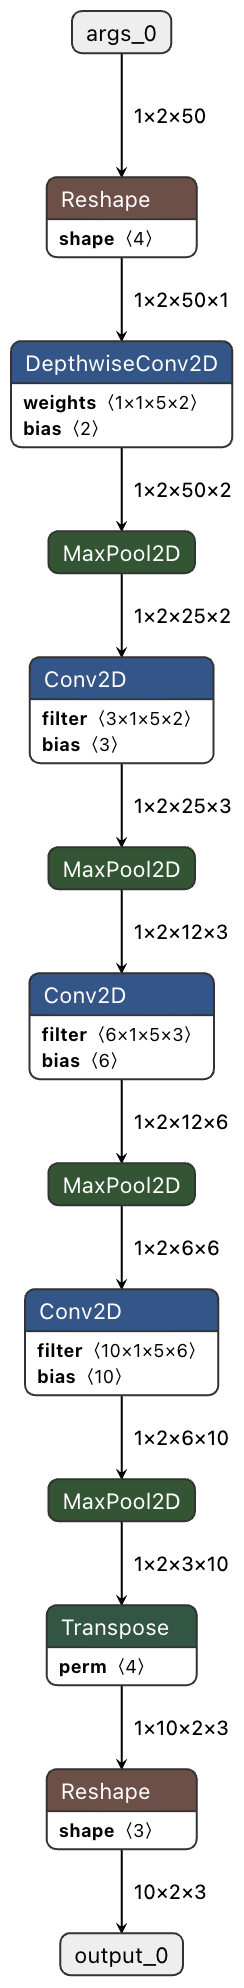
\includegraphics[width=0.7\textwidth]{Graphs/CONV-Graph-Layers-4}
      \caption{Figure shows Conv2D graph with 4 convolutional layers.}
      \label{fig:conv_graph}
    \end{figure}

    Across all Conv2D configurations, inference latency on internal SRAM is consistently
    lower than on PSRAM; for the $(1,40,40)$ input the float32 latency falls from
    $50534\,\mu s$ to $22606\,\mu s$ when the model is executed from SRAM. Int8
    quantization yields a further substantial reduction, lowering the same configuration
    from $50534\,\mu s$ (float32, PSRAM) to $15464\,\mu s$ (int8, PSRAM), a $3.27\times$
    speedup, at a negligible accuracy cost ($\mathrm{MSE}\leq0.0006$ throughout). The
    benefit of quantization is workload-dependent: for the smallest layer (a single
    output channel) int8 is marginally slower than float32 ($448\,\mu s$ vs.\
    $389\,\mu s$), whereas its relative advantage widens as the layer grows, reaching the
    $3.27\times$ factor noted above.

    Latency increases monotonically with input size, kernel size, and the number of
    output channels, as expected from the corresponding growth in the convolution
    workload. The layer-count sweep is the exception: because the architecture employs
    ``same'' convolutions with a MaxPool2D stage after each layer and assigns
    intermediate channel counts via geometric decay, each additional layer both halves
    the spatial extent of the feature map (Fig.~\ref{fig:conv_graph}, $50\!\to\!25\!\to\!
    12\!\to\!6$) and alters the distribution of intermediate channel widths. As a result,
    the per-layer cost falls rapidly with depth, and total latency is not monotonic in the
    number of layers; the four-layer model ($1556\,\mu s$, int8 PSRAM) is faster than the
    three-layer model ($1701\,\mu s$) because its intermediate channel allocation yields
    less work despite the additional stage.

    The memory footprint (Table~\ref{tab:conv_memory}) exhibits a clear separation between
    model size and arena (working-memory) requirements. Model size is largely insensitive
    to quantization for these small networks; because the parameter counts are modest, the
    per-tensor quantization metadata roughly offsets the four-fold reduction in weight
    precision, so int8 models are in fact marginally larger than their float32 counterparts
    for the smallest configurations (e.g.\ $2.3\,\mathrm{KB}\to2.6\,\mathrm{KB}$ for the
    single-layer $k{=}(1,5)$ model), and only become smaller once the weight tensors
    dominate (e.g.\ $3.3\,\mathrm{KB}\to2.8\,\mathrm{KB}$ at $k{=}(1,30)$). The arena, by
    contrast, is dominated by activation tensors and is where quantization delivers its
    principal benefit: for the $(1,40,40)$ input the arena falls from
    $119.6\,\mathrm{KB}$ (float32) to $30.5\,\mathrm{KB}$ (int8), a $3.9\times$ reduction.
    Arena size grows steeply with the activation volume, increasing with input size
    ($7.1\to119.6\,\mathrm{KB}$ for float32 as the input grows from $10\!\times\!10$ to
    $40\!\times\!40$) and with the number of output channels
    ($1.4\to23.4\,\mathrm{KB}$ from one to thirty channels), while remaining identical
    between the PSRAM and No-PSRAM configurations, confirming that memory placement
    affects latency but not footprint.

    \begin{table}[htbp]
      \centering
      \caption{LSTM layers performance on the ESP32-S3.}
      \label{tab:lstm_timing}
      \small
      \fittable{tables/lstm_timing.tex}
    \end{table}

    \begin{table}[htbp]
      \centering
      \caption{LSTM layers performance on the ESP32-S3.}
      \label{tab:lstm_memory}
      \small
      \fittable{tables/lstm_memory.tex}
    \end{table}
    \begin{figure}[H]
      \centering % Centers the image horizontally
      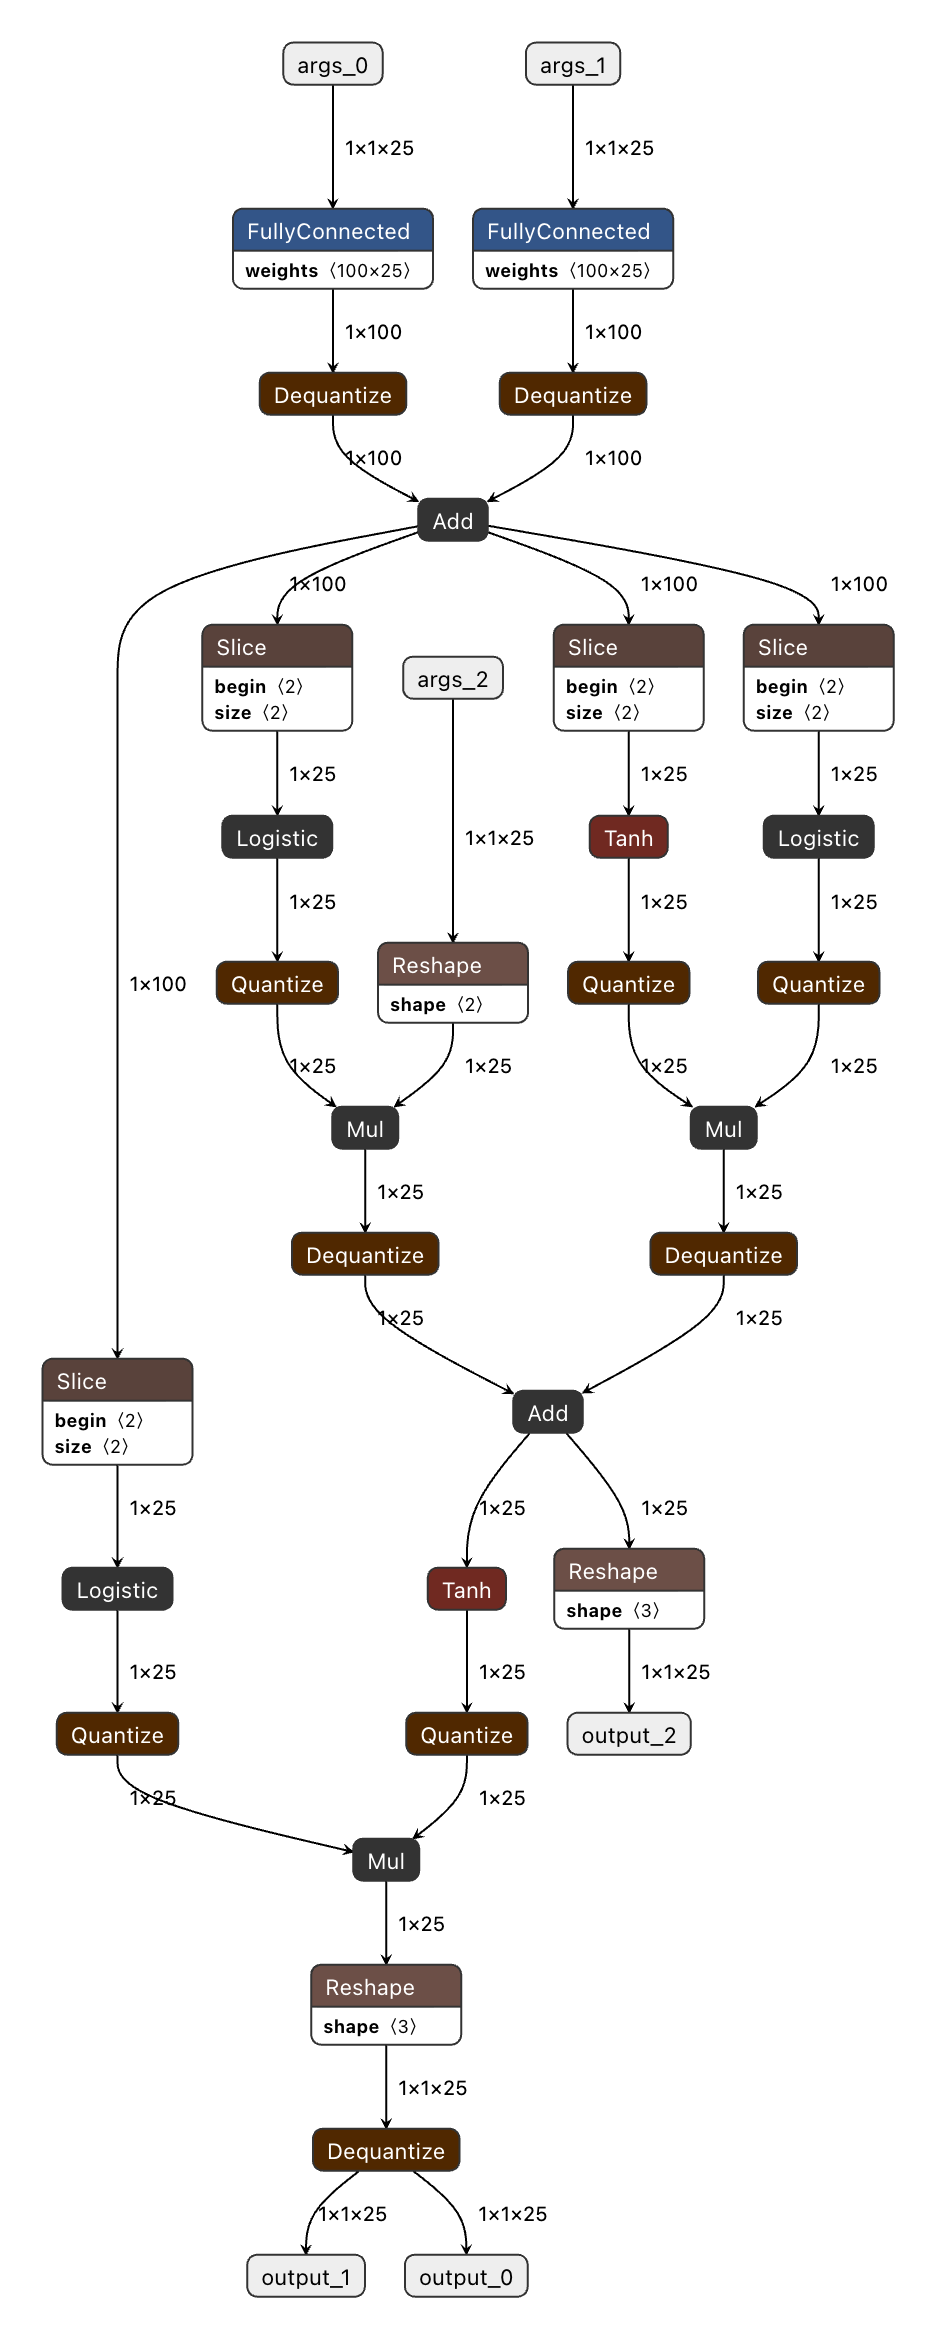
\includegraphics[width=0.7\textwidth]{Graphs/LSTM-Graph-25.png} % Omit the file extension
      \caption{Figure shows the accuracy of the quantization using the SQNR metric of Conv2D layers against Input size}
      \label{fig:lstm_graph_25}
    \end{figure}

  Table~\ref{tab:lstm_timing} reports our benchmark of the manually implemented LSTM
  layers using the default LiteRT export and quantization pipeline. Inspecting the
  exported model layout reveals that the dominant source of int8 latency overhead is
  the set of intermittent \texttt{Quantize}/\texttt{Dequantize} stages
  (Fig.~\ref{fig:lstm_graph_25}), which must traverse the entire activation tensors at
  each transition. The cost of these stages scales with the number of such traversals
  per inference: in the time-step and layer-count sweeps, where these transitions
  recur, int8 inference is consistently slower than its float32 counterpart (e.g.,
  $17538\,\mu s$ vs.\ $9542\,\mu s$ at $15$ time steps on PSRAM). Notably, this trend
  reverses for large single-layer hidden sizes, where the matrix computation dominates
  the quantization overhead and int8 becomes faster than float32 (e.g.,
  $27723\,\mu s$ vs.\ $42847\,\mu s$ for a hidden size of $200$ on PSRAM).

  A second observation concerns quantization quality. Single-layer, single-time-step
  configurations incur negligible error ($\mathrm{MSE}=0$), whereas accuracy degrades
  once additional time steps or stacked layers are introduced: the mean-squared error
  rises to $0.0036$ at $15$ time steps and reaches $0.0050$ for the four-layer
  configuration. This indicates that the accumulation of quantization error across
  recurrent and stacked computations, rather than the LSTM operation in isolation, is
  the principal driver of the observed accuracy loss.

  The memory footprint (Table~\ref{tab:lstm_memory}) shows the opposite balance to the
  convolutional case. Because LSTM weight matrices scale quadratically with the hidden
  size, the model is parameter-dominated, and int8 quantization produces large reductions
  in model size: for a hidden size of $200$ the model shrinks from
  $1256.2\,\mathrm{KB}$ (float32) to $340.0\,\mathrm{KB}$ (int8), a $3.7\times$
  saving. The arena, however, is consistently \emph{larger} under int8 than under
  float32 (e.g.\ $12.1\,\mathrm{KB}\to24.8\,\mathrm{KB}$ at hidden size $200$, and
  $31.6\,\mathrm{KB}\to85.9\,\mathrm{KB}$ at $20$ time steps), reflecting the additional
  scratch buffers required by the intermittent \texttt{Quantize}/\texttt{Dequantize}
  stages discussed above. Arena requirements also grow with the number of time steps
  ($3.2\to31.6\,\mathrm{KB}$ for float32 from one to twenty steps), which, together with
  the inflated int8 arena, explains why several int8 configurations exceed the available
  internal SRAM and could only be executed from PSRAM (denoted by dashes in
  Table~\ref{tab:lstm_timing}).
  \section{Comparison of different Model Configurations}  
  

  

    \begin{table}[htbp]
      \centering
      \caption{Model A (float32) performance on the ESP32-S3.}
      \label{tab:float32_model_A}
      \small
      \fittable{tables/float32_models_A/timing.tex}
    \end{table}

    \begin{table}[htbp]
      \centering
      \caption{Model A (int8 A,B, ELU stages) performance on the ESP32-S3.}
      \label{tab:int8_model_A}
      \small
      \fittable{tables/int8_models_A/timing.tex}
    \end{table}

    \begin{figure}[H]
      \centering % Centers the image horizontally
      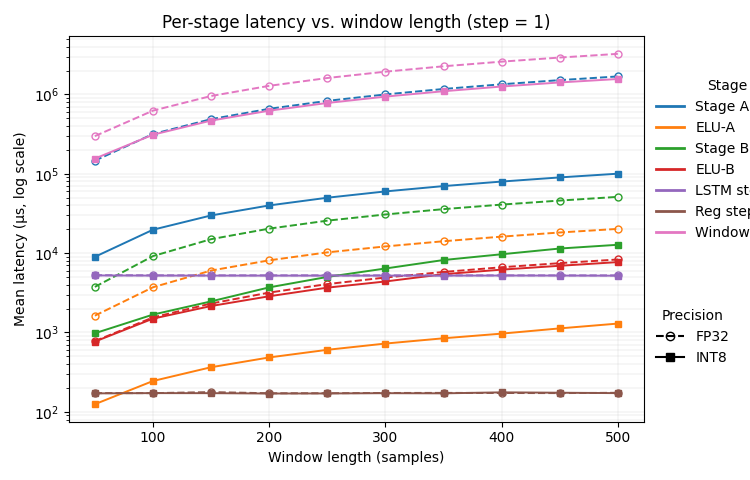
\includegraphics[width=0.7\textwidth]{Graphs/Per-Stage-Latency-Window-Log.png} % Omit the file extension
      \caption{Figure shows latency of model stages over window length.}
      \label{fig:conv2D_sqnr}
    \end{figure}

    \begin{figure}[H]
      \centering % Centers the image horizontally
      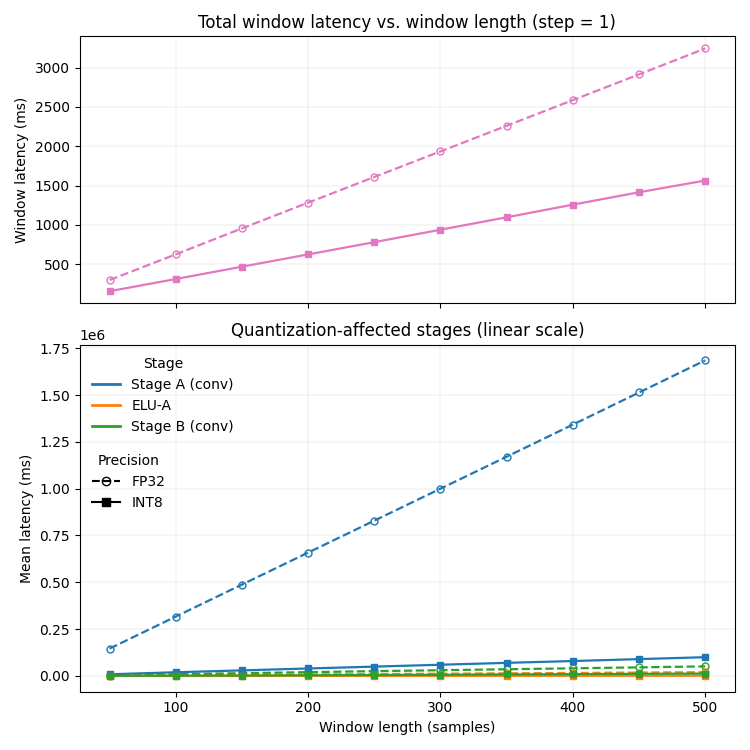
\includegraphics[width=0.7\textwidth]{Graphs/Per-Stage-Latency-Window-Linear.png} % Omit the file extension
      \caption{Figure shows latency of model stages over window length.}
      \label{fig:conv2D_sqnr}
    \end{figure}

    \begin{table}[htbp]
      \centering
      \caption{Model B (float32) performance on the ESP32-S3.}
      \label{tab:float32_model_B}
      \small
      \fittable{tables/float32_models_B/timing.tex}
    \end{table}

    \begin{table}[htbp]
      \centering
      \caption{Model B (int8 A,B, ELU stages) performance on the ESP32-S3.}
      \label{tab:int8_model_B}
      \small
      \fittable{tables/int8_models_B/timing.tex}
    \end{table}

\chapter{Discussion}
  \section{Model Performance}

The results confirm that \texttt{int8} quantization yields substantial latency
reductions for the convolutional inference stages on the ESP32-S3. Comparing the
fully floating-point configuration (Table~\ref{tab:float32_model_A}) with the
\texttt{int8} configuration (Table~\ref{tab:int8_model_A}), the Stage~A inference
cost falls from approximately $146{,}269$ to $8{,}983$ profiler ticks at a window
length of $50$, a speed-up of roughly $16\times$, while Stage~B improves by a
factor of about $3.8\times$. This disparity reflects the substantial gap between
the integer arithmetic units and the floating-point unit on the ESP32-S3, and is
further attributable to the ESP-NN backend, whose assembly-optimized kernels on
this platform target \texttt{int8} operations exclusively, leaving floating-point
paths to the generic, unoptimized implementations. As expected, quantization
introduces a measurable degradation in numerical fidelity: the mean squared error
rises from the order of $10^{-14}$ in the floating-point model---a value
consistent with floating-point rounding noise rather than algorithmic error---to
the range of approximately $8.0\times10^{-6}$ to $1.7\times10^{-4}$ under
\texttt{int8} quantization. We argue that this degradation remains tolerable given
the magnitude of the accompanying latency improvements.

The ELU activations represent a second area of concern. The TensorFlow Lite Micro
runtime and the ESP-NN backend implement only a limited set of activation
functions (such as ReLU, Hard-Swish, Logistic, and Softmax) and provide no native
implementation for ELU. Consequently, the LiteRT converter decomposes the
\texttt{torch.nn.ELU} module into a sequence of primitive operations. In the
quantized graph, the exporter further isolates this region as a floating-point
island bracketed by quantization and dequantization stages that traverse the
entire activation tensor, adding considerable overhead. To address this, we
removed the ELU section from the model graph and reimplemented it manually using
an \texttt{int8} look-up table (LUT). For the first activation block (ELU-A), this
substitution reduces the latency from approximately $1{,}630$ to $125$~\textmu s
at a window length of $50$ and from $20{,}211$ to $1{,}295$~\textmu s at a window
length of $500$, corresponding to a speed-up of roughly $13$ to $16\times$. We
note that the second activation block (ELU-B) is retained in floating point
(dequantized from \texttt{int8} without a LUT) and therefore exhibits no
comparable improvement, with its latency remaining essentially unchanged between
the two configurations (for example, $779$ versus $768$~\textmu s at a window
length of $50$).

The LSTM step size constitutes an important hyperparameter governing the trade-off
between recurrent loop overhead and memory footprint. Because the multi-layer LSTM
is unrolled into its constituent operations, retaining all unrolled timesteps is
infeasible: the activation arena grows rapidly with the number of timesteps
processed per invocation. This increase affects not only the static memory
footprint but potentially the latency as well, since larger arenas may require
allocation in the slower external PSRAM or flash, incurring additional
memory-access latency. Increasing the step size batches more timesteps into shared
buffers, thereby amortizing the recurrent loop overhead. In our measurements,
raising the LSTM step size from $1$ to $5$ approximately triples the arena reserved
for the LSTM stage, from $8.86$ to $24.77$~kB (a factor of $2.79$). The step size
must therefore be tuned to the deployment scenario and the data dimensionality at
hand in order to maximize performance within a tolerable memory budget.

Window length plays a decisive role in overall pipeline latency and is arguably
the single most influential contributor to the end-to-end timing. Our results
demonstrate a near-linear relationship between window length and the time required
to produce an inference over a complete window: in the floating-point configuration,
the mean per-window latency increases from approximately $298{,}232$~\textmu s at a
window length of $50$ to $3{,}244{,}354$~\textmu s at a window length of $500$,
corresponding to an essentially constant per-sample cost of roughly $6{,}000$~\textmu s.

Finally, our results indicate that quantization of the LSTM and regression stages
is counterproductive, offering minimal returns relative to the implementation
difficulty. Unlike feed-forward architectures such as dense and convolutional
layers, the LSTM is recurrent: its output at a given timestep feeds the
computation at the next, which causes quantization error to compound across
timesteps, so that even small errors at the initial timestep accumulate into
substantial deviations at the final output. The same effect applies to the
regression head, which is invoked within the same recurrent loop. Cell-state
quantization is particularly problematic. In contrast to the hidden state, the
cell state exhibits a wide dynamic range---spanning approximately $-30$ to $30$ in
our experiments---which causes standard \texttt{int8} quantization to be coarse:
numerically significant variations are collapsed into narrow ranges, producing
repeated saturated values and severely degraded error metrics. The conventional
remedy is a dedicated \texttt{int16} quantization scheme for the cell-state path,
which is supported neither by the LiteRT converter nor by the ESP-NN kernels. This
would require hand-written operations for the elementwise multiplications and
additions, together with more memory-intensive LUTs for activations such as
$\tanh$ ($64$~kB each, compared with $256$~bytes for \texttt{int8} data). The
literature on LSTM quantization remains sparse, with the few available studies
recommending quantization-aware training methods, which lie beyond the scope of
this work.

\chapter{Conclusion}
  \section{Conclusion}

  \section{Limitations}
  Several limitations of this work merit discussion.

  First, the scope of this thesis was confined to the implementation of the
  provided model architecture, which was adopted without modification. This is a
  relevant consideration, as it has been argued that purely convolutional (TCN)
  architectures can be more reliable than recurrent (RNN) architectures for
  capturing temporal dependencies in sEMG data \cite{zanghieriRobustRealTimeEmbedded2020};
  a systematic comparison between the two paradigms on the target hardware therefore
  remains outside the scope of the present work.

  Second, we deliberately adopted a cross-platform approach, seeking to avoid
  tying the pipeline to any single hardware target. Although all experiments were
  conducted on ESP32 chips, the pipeline is readily generalisable, as it relies on
  the industry-standard LiteRT framework. While LiteRT and TensorFlow Lite Micro
  map operations to native kernel backends, the final performance could nonetheless
  benefit substantially from platform-specific optimisations that this work did not pursue.

  Third, although several LSTM quantisation schemes were investigated, none yielded
  reliable results. This outcome is attributable to a number of factors that warrant
  further investigation before faster and more dependable quantisation of recurrent
  layers can be achieved.

  Finally, because the model was supplied pre-trained, quantisation-aware training (QAT)
  was not explored in depth. Several studies nonetheless report considerable benefits of
  QAT over simpler post-training quantisation (PTQ) schemes, suggesting a promising
  direction for improvement. Additionally, alternative quantisation schemes such as hybrid
  and int16 quantisation were not examined, owing to their incompatibility with the
  Espressif platforms targeted in this work.

\section{Future Work}
  The limitations identified above suggest several promising directions for future research.

  First, the deployment pipeline could be evaluated across a broader range of model
  architectures. In particular, a systematic comparison between the recurrent (LSTM-based)
  model studied here and a purely convolutional (TCN) counterpart, conducted directly on the
  target hardware, would clarify the trade-offs between accuracy, memory footprint, and
  inference latency for each paradigm under realistic embedded constraints.

  Second, while the cross-platform design of the pipeline favours portability, future work
  could quantify the performance gains attainable through platform-specific optimisation.
  Deploying the pipeline on hardware with dedicated neural-network acceleration, or
  substituting hand-optimised kernels for the default backend, would establish how much
  additional efficiency can be recovered without sacrificing the framework's generality.

  Third, the difficulties encountered in quantising the recurrent layers motivate a dedicated
  investigation into reliable quantisation of LSTM and other RNN-based components. Identifying
  the sources of instability, and developing or adopting quantisation strategies tailored to
  recurrent computation, would directly address one of the central implementation challenges
  of this work.

  Finally, the quantisation methodology itself could be extended. Incorporating
  quantisation-aware training (QAT), provided the training pipeline is made available, may
  yield accuracy improvements over the post-training quantisation employed here. Likewise,
  evaluating alternative schemes such as hybrid and int16 quantisation on hardware platforms
  that support them would help characterise the full design space of accuracy-versus-efficiency
  trade-offs for embedded sEMG regression.

\appendix
\chapter{Additionally}
% -------------------> end writing here <------------------------
% *****************************************************************
\listoffigures
\listoftables

\ifthenelse{\equal{\doclang}{german}}{
	\bibliographystyle{IEEEtran_ISSger}
}{
	\bibliographystyle{IEEEtran_ISS}
}
\bibliography{refs}

% *****************************************************************
%% Additional page with Declaration ("Eidesstattliche Erklrung");
%% completed automatically
\begin{titlepage}
      \vfill
      \LARGE \ifthenelse{\equal{\doclang}{german}}{\textbf{Erkl\"arung}}{\textbf{Declaration}}
      \vfill

      \ifthenelse{\equal{\doclang}{german}}{
         Hiermit erkl\"are ich, dass ich diese Arbeit selbstst\"andig verfasst und keine anderen als die angegebenen
         Quellen und Hilfsmittel benutzt habe.
      }
      {
         Herewith, I declare that I have developed and written the enclosed thesis entirely by myself and that I have not used sources or means except those declared.
      }

      \vspace{1cm}

      \ifthenelse{\equal{\doclang}{german}}{
         Die Arbeit wurde bisher keiner anderen Pr\"ufungsbeh\"orde vorgelegt und auch noch nicht ver\"offentlicht.
      }
      {
         This thesis has not been submitted to any other authority to achieve an academic grading and has not been published elsewhere.
      }

      \vfill

      
      Stuttgart, \signagedate
      \hfill
      \begin{tabular}{l}
          \hline
          \student
      \end{tabular}
\end{titlepage}



\end{document}
